\chapter{测度}
\label{chap:measure-spaces}
\label{chap:measures}

数一个有限集合有几个元素，量一条线段有多长，称一批货物有多重，回答的都是“这一部分有多大”。这些量有一个共同的规则：把对象分成互不相交的几部分，整体的大小等于各部分大小之和。可是一旦集合变得复杂，例如区间里的全部有理点、无限次挖去中间三分之一后剩下的点集，单凭有限个区间去逼近就不再能给出可靠的答案。本章的目标是把“分开测量、合起来相加”的规则推广到可数次分割，建立测度这一对象，并回答三个问题：怎样测量集合，怎样经过映射传递质量，怎样比较与分解不同的测度。

第~\ref{sec:measure-size-additivity}节从计数、长度与Jordan测量出发，用有理点集说明有限区间逼近的局限，提出对可数运算的要求。第~\ref{sec:measure-spaces-def}节把“哪些集合允许测量”与“怎样赋予大小”分开，建立$\sigma$代数、Borel集、测度及零测集；第~\ref{sec:measure-construction}节再回答测度从何而来，用外测度构造实轴上的Lebesgue测度和Lebesgue--Stieltjes测度，并证明在生成族上一致的测度何时处处一致。第~\ref{sec:measure-measurable-maps}节用原像定义可测映射与可测函数，第~\ref{sec:measure-pushforward}节固定一个可测映射，研究输入质量怎样汇集到输出集合上。

后三节在同一可测空间上比较测度。第~\ref{sec:measure-relations}节用零测集刻画绝对连续与相互奇异；第~\ref{sec:measure-signed}节允许两个测度相减，建立有符号测度的Hahn分解、Jordan分解与总变差；第~\ref{sec:measure-decomposition}节相对于参考测度把一个测度拆成绝对连续部分与奇异部分，并在实轴上分出点质量、绝对连续质量与奇异连续质量。第~\ref{sec:measure-summary}节回顾这些结构的分工。本章只使用集合运算、可数性与级数，不依赖积分：积分在第~\ref{chap:integration}章建立，用密度表示测度的问题留到第~\ref{chap:densities-change-of-measure}章。

\section{集合大小与可加性}
\label{sec:measure-size-additivity}

测度要推广的是我们已经会做的两件事：数有限集合的元素，量区间的长度。本节先从这两种测量中提取共同的相加规则，再用有限个区间去逼近一般集合，得到Jordan测量。有理点集的例子将说明，只允许有限个区间会让一些很“稀疏”的集合得到不合理的大小；改用可数个区间以后，问题就转化为要求测量规则对可数运算封闭、对可数分割可加。

\subsection{计数与长度}
\label{sec:measure-counting-length}

\paragraph{计数与加权计数}
对有限集合$A$，用$\#A$表示它的元素个数。若$A$与$B$不相交，合并后的元素恰好被数了一次，所以$\#(A\cup B)=\#A+\#B$。更一般地，给有限集合$X$的每个点$x$配一个非负权重$w_x$，令$A\subseteq X$的大小为$\sum_{x\in A}w_x$，不相交集合合并时仍然是各部分权重之和。权重全取$1$时就是计数；权重不同时，大小不再等于元素个数，例如质量、费用或频率。

图~\ref{fig:measure-count-length}(a)中$X=\{1,2,3,4,5\}$，权重依次为$0.5,1,2,0.5,1$。分组$A=\{1,2,3\}$、$B=\{4,5\}$后，$A$的元素个数为$3$、总权重为$3.5$，$B$的元素个数为$2$、总权重为$1.5$；整体的个数$5=3+2$，总权重$5=3.5+1.5$。两种大小的数值不同，但遵守同一条规则：不交的部分相加得到整体。

\paragraph{区间长度}
换成实轴上的区间，元素已经无法逐个数完。对端点为$a\le b$的区间，不论端点是否属于该区间，规定它的长度为$b-a$，记作$\ell$。任意两个非退化区间都与$\mathbb R$等势（可参考\BookChapterRef{chap:cardinality}{卷一“基数”章}），按元素个数无法区分$[0,1]$与$[0,2]$，长度却分别为$1$和$2$。所以长度度量的是集合在实轴上占据的范围，而不是元素的多少。后面的测度同样是给集合赋予大小的规则，计数只是其中一种。

\paragraph{有限个不交区间的长度}
设$E$是有限个两两不交区间$I_1,\dots,I_m$的并，自然规定$\ell(E)=\sum_{k=1}^m\ell(I_k)$。同一个$E$往往有多种分割方式，这个定义要有意义，必须先说明结果与分割方式无关。取两种分割的全部端点，从小到大排列，它们把每个区间切成若干相邻的小区间，得到两种分割的\emph{共同细分}。一个区间被切点$a=t_0<t_1<\dots<t_r=b$分开后，小区间长度之和$\sum_{j}(t_j-t_{j-1})=b-a$逐项相消，等于原长度；因此两种分割的长度和都等于共同细分的长度和。

图~\ref{fig:measure-count-length}(b)中$E=[0,2)\cup[3,4)$。第一种分割为$[0,1.5),[1.5,2),[3,4)$，长度和为$1.5+0.5+1=3$；第二种为$[0,0.5),[0.5,2),[3,3.5),[3.5,4)$，长度和为$0.5+1.5+0.5+0.5=3$。共同细分的切点是$0,0.5,1.5,2,3,3.5,4$，两种分割的每个区间都是若干细分小区间之并，所以得到相同的总长度。

\begin{figure}[!htbp]
  \centering
  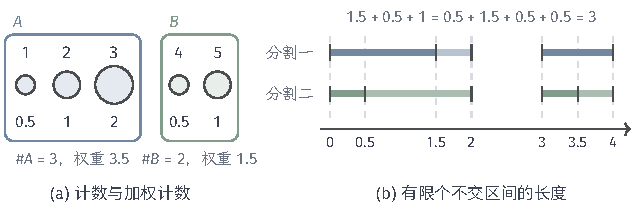
\includegraphics[width=107.6mm]{figures/02-abstract-mathematics/01-metric-and-measure/tikz/c2-count-length/figure.pdf}
  \caption{计数、加权计数与长度遵守同一条不交相加规则。(a)五个点按权重画成大小不同的圆，分成$A=\{1,2,3\}$与$B=\{4,5\}$后，个数$3+2=5$，总权重$3.5+1.5=5$；(b)集合$E=[0,2)\cup[3,4)$的两种不交区间分割，灰色竖线是共同细分的切点，两种分割的长度和都等于$3$。}
  \label{fig:measure-count-length}
\end{figure}

\paragraph{有限的含义}
这里的“有限”限制的是参与分割的区间个数，每个区间中仍有无限多个点。非退化区间不能写成有限个单点的并，因此有限可加性既不会在单点层面产生矛盾，也不提供关于单点分割的任何信息。如果把$[0,1]$看成全部单点$\{x\}$的并，每个单点长度为$0$，而“$0$的不可数和”没有定义，有限可加性根本不适用于这种分割。后面将看到，测度允许的是可数分割：比有限分割多，又比任意不可数分割少，这条界线正是后续理论成立的依据。

\subsection{Jordan测量}
\label{sec:measure-jordan}

有限个不交区间的并只是很少一部分集合。对更一般的有界集合，自然的想法是从里面和外面同时用这类简单集合去逼近。下面把有限个有界区间的并称为\term{初等集合}（elementary set）；它总能改写成有限个不交区间的并，因此上一小节的长度对它有定义。若初等集合$P\subseteq Q$，则$Q\setminus P$仍是初等集合，于是$\ell(P)\le\ell(P)+\ell(Q\setminus P)=\ell(Q)$，长度对包含关系单调；对任意两个初等集合，再由$P\cup Q=P\cup(Q\setminus P)$得$\ell(P\cup Q)\le\ell(P)+\ell(Q)$，并可推广到有限个。

\begin{definition}[Jordan测量]
\label{def:measure-jordan}
设$E\subseteq\mathbb R$有界。称
\[
 \begin{aligned}
  J_*(E)&=\sup\{\ell(P):P\text{为初等集合},\ P\subseteq E\},\\
  J^*(E)&=\inf\{\ell(Q):Q\text{为初等集合},\ E\subseteq Q\}
 \end{aligned}
\]
分别为$E$的\term{Jordan内测量}（Jordan inner content）与\term{Jordan外测量}（Jordan outer content），其中空集作为初等集合长度为$0$。若$J_*(E)=J^*(E)$，称$E$是\term{Jordan可测}（Jordan measurable）的，公共值记为$J(E)$，称为$E$的\term{Jordan测量}（Jordan content）。
\end{definition}

任取内部初等集合$P\subseteq E$与外部初等集合$Q\supseteq E$，有$P\subseteq Q$，由单调性得$\ell(P)\le\ell(Q)$，所以总有$J_*(E)\le J^*(E)$。Jordan可测就是内外两侧可以夹逼到同一个数。这与卷一用有限分割上的上和、下和夹逼定积分是同一种思路（可参考\BookChapterRef{chap:univariate-integration}{卷一“一元积分”章}）：那里固定区间、逼近函数下方的面积，这里固定长度规则、逼近集合本身。

\paragraph{Jordan可测集的例子}
区间$[a,b]$本身是初等集合，内外测量都等于$b-a$。有限个区间的并同理。边界简单的无限集合也可以Jordan可测：取$E=\{1/n:n\ge1\}$，它不含非退化区间，内测量为$0$；对任意$N$与$\varepsilon>0$，用$[0,1/N]$盖住$n\ge N$的全部点，再用长度各为$\varepsilon/N$的小区间盖住$1,1/2,\dots,1/(N-1)$，外部初等集合的长度不超过$1/N+\varepsilon$，令$N\to\infty$、$\varepsilon\to0$得$J^*(E)=0$。可见有限个区间可以覆盖无限多个点，前提是这些点聚集在少数位置附近。

\paragraph{有理点集的反例}
取$E=\mathbb Q\cap[0,1]$。任何非退化区间都含无理数，所以包含在$E$中的初等集合只能由单点组成，长度为$0$，$J_*(E)=0$。另一方面，设初等集合$Q\supseteq E$，把它写成不交区间$I_1,\dots,I_m$的并。把每个$I_k$换成它的闭包$\overline{I_k}$，长度不变，而$\bigcup_k\overline{I_k}$是闭集并包含$E$；$E$在$[0,1]$中稠密，所以这个闭集包含$E$的全部极限点，即包含$[0,1]$。由有限次可加与单调性，$\ell(Q)=\sum_k\ell(\overline{I_k})\ge\ell(\bigcup_k\overline{I_k})\ge\ell([0,1])=1$；而$[0,1]$本身是外部初等集合，故$J^*(E)=1$。内外测量分别为$0$和$1$，$E$不是Jordan可测的。问题出在有限覆盖：有理点到处都是，有限个区间要盖住它们，就不得不连同中间的全部无理数一起盖住。

如果允许可数个区间，情况完全不同。把$E$中的点排成一列$q_1,q_2,\dots$，对给定的$\varepsilon>0$，用长度为$\varepsilon2^{-k}$、以$q_k$为中心的开区间盖住$q_k$。这些区间盖住了$E$，长度总和为$\sum_{k\ge1}\varepsilon2^{-k}=\varepsilon$。图~\ref{fig:measure-jordan-rationals}对比了两种覆盖：有限覆盖必须铺满整个$[0,1]$，可数覆盖的区间越来越短，总长可以任意小。可数覆盖于是给出了另一种测量方式，在它之下有理点集的大小应为$0$。

\begin{figure}[!htbp]
  \centering
  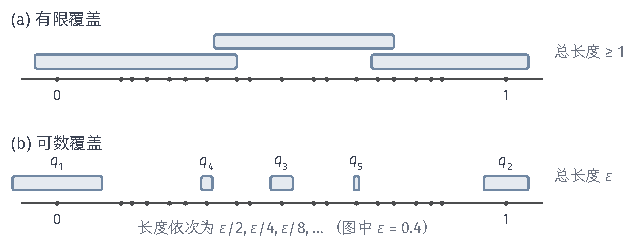
\includegraphics[width=107.8mm]{figures/02-abstract-mathematics/01-metric-and-measure/tikz/c2-jordan-rationals/figure.pdf}
  \caption{用区间覆盖$[0,1]$中的有理点。(a)有限个区间要盖住稠密的有理点，闭包后必须铺满$[0,1]$，总长度不小于$1$；(b)按排列顺序给第$k$个有理点$q_k$分配长度$\varepsilon2^{-k}$的区间，图中只画出前五个，长度依次减半，总长度为$\varepsilon$。}
  \label{fig:measure-jordan-rationals}
\end{figure}

\paragraph{对可数运算的要求}
有理点集还暴露了Jordan测量的另一缺陷。每个单点$\{q_k\}$都Jordan可测且测量为$0$，可是它们的可数并$E$不是Jordan可测的；Jordan可测集合族对可数并不封闭。然而分析中处处需要可数运算：一列集合取并或取交，用逐项逼近得到的集合列求极限，把一个集合分成可数个不交的部分。我们因此提出两项要求。第一，允许测量的集合族应对补集、可数并和可数交封闭；第二，若集合被分成可数个不交的可测部分，整体的大小应等于各部分大小的级数和。这里只提出要求，满足它们的测量规则是否存在、与区间长度是否一致，由第~\ref{sec:measure-construction}节的构造回答。

\section{测度空间}
\label{sec:measure-spaces-def}

上一节提出的两项要求分别针对不同对象：一项限定哪些集合允许测量，另一项规定怎样给这些集合赋予大小。本节把它们分开建立。先用$\sigma$代数描述允许测量的集合族，在度量空间上由开集得到Borel集；再在其上定义可数可加的测度，推出比较、取极限与加权的规则；最后讨论哪些例外可以忽略，以及怎样把零测集的子集纳入可测范围。

\subsection{$\sigma$代数}
\label{sec:measure-sigma-algebras}

\paragraph{能够区分哪些集合}
设$X=\{1,2,3,4\}$。若允许测量全部$16$个子集，就能单独询问每个点的大小；若只知道每个点属于$\{1,2\}$还是$\{3,4\}$，能够回答的只有$\varnothing$、$\{1,2\}$、$\{3,4\}$、$X$这四个集合是否发生，单点$\{1\}$无法单独测量。两种集合族底集相同，区分能力不同。无论选哪一种，只要$A$允许测量，“不在$A$中”也应允许测量；只要一列集合都允许测量，“至少属于其中一个”也应允许测量。这正是上一节对可数运算的要求。

\begin{definition}[$\sigma$代数]
\label{def:measure-sigma-algebra}
设$X$是集合，$\mathcal A$是$X$的一族子集。若
\begin{enumerate}
 \item $X\in\mathcal A$；
 \item $A\in\mathcal A$蕴含$X\setminus A\in\mathcal A$；
 \item $A_1,A_2,\dots\in\mathcal A$蕴含$\bigcup_{n\ge1}A_n\in\mathcal A$，
\end{enumerate}
则称$\mathcal A$为$X$上的一个\term{$\sigma$代数}（sigma-algebra），称$(X,\mathcal A)$为\term{可测空间}（measurable space），称$\mathcal A$中的集合为\term{可测集合}（measurable set）。
\end{definition}

定义只列出补集与可数并，其他运算由它们得到。由第1、2条，$\varnothing=X\setminus X\in\mathcal A$；在第3条中从某项起全取$\varnothing$，得到有限并封闭。可数交由De Morgan律化为补集与并：
\[
 \bigcap_{n\ge1}A_n=X\setminus\bigcup_{n\ge1}(X\setminus A_n),
\]
差集$A\setminus B=A\cap(X\setminus B)$也属于$\mathcal A$。所以从可测集合出发，经可数次补、并、交、差得到的集合仍然可测。开头的两种集合族都满足这些条件：幂集$\mathcal P(X)$含全部子集，任何运算结果都仍在其中；四个集合$\{\varnothing,\{1,2\},\{3,4\},X\}$中任一个的补集仍在其中，任意几个的并也在其中。

\paragraph{生成的$\sigma$代数}
实际问题中我们通常只点名少数必须能测量的集合，例如区间或若干类别，希望由它们补齐其余集合。给定$X$的一族子集$\mathcal C$，包含$\mathcal C$的$\sigma$代数至少有幂集一个。令$\sigma(\mathcal C)$为所有包含$\mathcal C$的$\sigma$代数之交，称为$\mathcal C$\term{生成的$\sigma$代数}（generated sigma-algebra）。逐条核对：每个参与求交的$\sigma$代数都含$X$，对补集、可数并封闭，交集中的元素同时属于它们全体，运算结果也同时属于它们全体，所以$\sigma(\mathcal C)$是$\sigma$代数；它包含$\mathcal C$，又包含于任何包含$\mathcal C$的$\sigma$代数，因此是其中最小的一个。

\begin{example}[有限分组生成的$\sigma$代数]
\label{ex:measure-partition-sigma}
在$X=\{1,2,3,4\}$上取$\mathcal C=\{\{1\},\{2\}\}$。生成的$\sigma$代数必须含$\{1\}$、$\{2\}$以及$X\setminus(\{1\}\cup\{2\})=\{3,4\}$，于是含有分组$\{1\},\{2\},\{3,4\}$中任意几组的并，共$2^3=8$个集合。这$8$个集合对补集和并已经封闭，所以它们就是$\sigma(\mathcal C)$；$\{3\}$不在其中。一般地，有限集合被分成$k$组时，由各组生成的$\sigma$代数恰由若干组之并组成，共$2^k$个集合。图~\ref{fig:measure-partition-sigma}比较了三种分组：组分得越细，可以单独测量的集合越多。
\end{example}

\begin{figure}[!htbp]
  \centering
  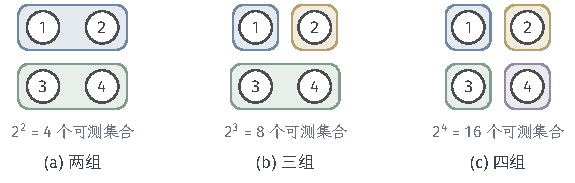
\includegraphics[width=97.3mm]{figures/02-abstract-mathematics/01-metric-and-measure/tikz/c2-sigma-algebra-partition/figure.pdf}
  \caption{四点集合$X=\{1,2,3,4\}$上由分组生成的$\sigma$代数。每个色块是一组，可测集合恰是若干组之并。(a)分成$\{1,2\},\{3,4\}$两组，得到$2^2=4$个可测集合；(b)分成$\{1\},\{2\},\{3,4\}$三组，得到$2^3=8$个；(c)每点自成一组，得到全部$2^4=16$个子集。}
  \label{fig:measure-partition-sigma}
\end{figure}

生成操作补齐的只是可数运算的封闭性，未必得到所有希望测量的集合。在$\mathbb R$上取全体单点组成的族$\mathcal C$。令$\mathcal D$为$\mathbb R$中可数集合与补集可数的集合的全体：它含$\mathbb R$；可数集的补集补集可数，反之亦然；一列集合若都可数，并可数，若有一个补集可数，并的补集包含于它的补集，也可数。所以$\mathcal D$是含全部单点的$\sigma$代数，$\sigma(\mathcal C)\subseteq\mathcal D$。而$[0,1]$与它的补集都不可数，$[0,1]\notin\mathcal D$。因此单点生成的$\sigma$代数不含任何区间，要测量区间，生成族里必须直接放入区间或开集。

\paragraph{迹$\sigma$代数与子$\sigma$代数}
改变“可测范围”有两种不同的操作。第一种缩小底集：设$Y\subseteq X$，令$\mathcal A_Y=\{A\cap Y:A\in\mathcal A\}$。由$(A\cap Y)$在$Y$中的补集为$(X\setminus A)\cap Y$，以及$\bigcup_n(A_n\cap Y)=(\bigcup_nA_n)\cap Y$，它是$Y$上的$\sigma$代数，称为\term{迹$\sigma$代数}（trace sigma-algebra）。第二种保持底集不变、只保留一部分可测集合：若$\mathcal G\subseteq\mathcal A$本身也是$X$上的$\sigma$代数，称$\mathcal G$为$\mathcal A$的\term{子$\sigma$代数}（sub-sigma-algebra）。

仍取$X=\{1,2,3,4\}$与$\mathcal A=\mathcal P(X)$。迹$\sigma$代数$\mathcal A_{\{1,2\}}=\mathcal P(\{1,2\})$丢掉了点$3,4$，剩下的点仍可逐个区分；子$\sigma$代数$\mathcal G=\{\varnothing,\{1,2\},\{3,4\},X\}$保留全部四个点，却只能分辨它们属于哪一组。前者改变研究对象，后者改变对同一批对象的分辨精度。后面讨论“只掌握部分信息”时，所用的正是子$\sigma$代数。

\subsection{Borel $\sigma$代数}
\label{sec:measure-borel-sets}

\paragraph{由开集生成}
在度量空间中已经有一族自然的集合：开集。第~\ref{sec:metric-open-closed}节用开球定义了开集与闭集，连续性、收敛与紧性都通过它们表达。把开集作为生成族，就得到与这些结构相容的可测范围。

\begin{definition}[Borel $\sigma$代数]
\label{def:measure-borel}
设$(X,d)$是度量空间。由全体开集生成的$\sigma$代数称为$X$的\term{Borel $\sigma$代数}（Borel sigma-algebra），记作$\mathcal B(X)$，其中的集合称为\term{Borel集}（Borel set）。
\end{definition}

开集的补集是闭集，所以闭集都是Borel集；可数个闭集的并、可数个开集的交也是Borel集。例如$\mathbb Q$是可数个闭集$\{q\}$的并，$[0,1)=\bigcap_{n\ge1}(-1/n,1)$是可数个开集的交，二者都是Borel集。需要强调，$\mathcal B(X)$只规定了哪些集合允许测量，并没有规定任何集合的大小；同一个Borel结构上可以放置长度、点质量或它们的组合等不同测度。

\paragraph{实轴上的生成族}
在$\mathbb R$上直接处理全部开集并不方便，下面说明较小的区间族已经足够。关键是把任意开集写成可数个区间的并。

\begin{lemma}[开集的有理区间表示]
\label{lem:measure-open-rational-intervals}
$\mathbb R$中每个开集$U$都是有理端点开区间的可数并。
\end{lemma}

\begin{proof}
任取$x\in U$。由$U$是开集，存在$r>0$使$(x-r,x+r)\subseteq U$。有理数在实轴上稠密，可以取有理数$p,q$满足$x-r<p<x<q<x+r$，于是$x\in(p,q)\subseteq U$。所以$U$等于所有包含于$U$的有理端点开区间$(p,q)$之并。这样的区间由有序对$(p,q)\in\mathbb Q\times\mathbb Q$确定，而$\mathbb Q\times\mathbb Q$可数，故这是一个可数并。
\end{proof}

\begin{theorem}[$\mathcal B(\mathbb R)$的生成族]
\label{thm:measure-borel-generators}
下列每一族集合都生成$\mathcal B(\mathbb R)$：(1)全体开区间$(a,b)$；(2)全体半直线$(a,+\infty)$；(3)全体半直线$(-\infty,a]$；(4)全体左开右闭区间$(a,b]$。在(2)(3)中只取有理数$a$也够用。
\end{theorem}

\begin{proof}
各族中的集合都是开集、闭集或二者的交，都属于$\mathcal B(\mathbb R)$，所以它们生成的$\sigma$代数都包含于$\mathcal B(\mathbb R)$。反向只需说明每个开集属于各族生成的$\sigma$代数。对族(1)，这正是引理~\ref{lem:measure-open-rational-intervals}。其余各族都能经可数运算得到开区间：取$\mathbb Q$中递减趋于$a$的序列$(p_n)$，有$(a,+\infty)=\bigcup_n(p_n,+\infty)$，所以端点为有理数的半直线已能生成族(2)中的全部半直线；$(-\infty,a]$的补集是$(a,+\infty)$，故族(3)与族(2)生成同一$\sigma$代数；$(a,b]=(-\infty,b]\setminus(-\infty,a]$，又$(a,b)=\bigcup_{n}(a,b-1/n]$（$n$取使$b-1/n>a$的整数），所以开区间属于族(3)或族(4)生成的$\sigma$代数；族(4)又通过$(a,+\infty)=\bigcup_n(a,a+n]$生成族(2)。
\end{proof}

\paragraph{开集的不交区间分解}
引理~\ref{lem:measure-open-rational-intervals}中的区间通常互相重叠。后面构造长度测度时，更方便的是把开集拆成互不相交的区间。对开集$U\subseteq\mathbb R$与$x,y\in U$，若$x$与$y$之间的闭区间整个含于$U$，记$x\sim y$。这个关系自反、对称；若$x\sim y$、$y\sim z$，连接$x,z$的区间含于连接$x,y$与连接$y,z$的两个区间之并，所以也传递。每个等价类$C$都具有“两点之间的点仍在其中”的性质，因而是区间；对$x\in C$，$U$中以$x$为中心的小开区间内各点都与$x$等价，所以$C$是开区间。不同等价类互不相交，在每一类中各取一个有理数，就得到从这些类到$\mathbb Q$的单射，因此类至多可数。这样，$\mathbb R$中每个开集都是至多可数个互不相交开区间的并，这些区间称为$U$的\term{连通分量}（connected component）。

图~\ref{fig:measure-open-set-components}中$U=(0,1)\cup(1,2)\cup(2.5,4)$。点$1$不在$U$中，所以$0.5$与$1.5$不等价；$U$恰分成三个分量，分别含有理数$1/2$、$3/2$、$3$。后面一旦知道测度在区间上的取值，就能借这个分解控制它在开集上的取值。

\begin{figure}[!htbp]
  \centering
  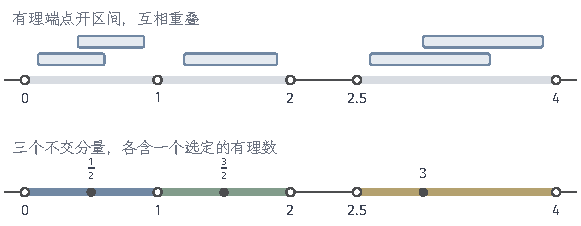
\includegraphics[width=98.4mm]{figures/02-abstract-mathematics/01-metric-and-measure/tikz/c2-open-set-components/figure.pdf}
  \caption{开集$U=(0,1)\cup(1,2)\cup(2.5,4)$的两种区间表示。上行：$U$中若干有理端点开区间，它们互相重叠，全体有理端点区间之并恰为$U$；下行：按“两点之间的闭区间是否含于$U$”分类得到三个互不相交的分量，每个分量中选一个有理数（圆点），说明分量至多可数。}
  \label{fig:measure-open-set-components}
\end{figure}

\paragraph{离散空间}
若$X$是有限集或可数集，并且每个单点都是闭集（例如带离散度量，或$\mathbb N$作为$\mathbb R$的子空间），那么任一子集$A$都是可数个闭单点的并，属于$\mathcal B(X)$，即$\mathcal B(X)=\mathcal P(X)$。在这类空间上，测量任意子集都不受限制，下面的计数测度和加权点测度直接以全部子集为可测范围。第~\ref{chap:integration}章将看到，离散空间上的积分就是加权求和，连续情形与离散情形由此纳入同一种形式。

\subsection{测度的定义}
\label{sec:measure-definition}

可测范围确定以后，需要给每个可测集合配一个非负的大小，并要求上一节提出的可数可加性成立。允许取值$+\infty$，是因为整条实轴的长度、无限集合的元素个数都没有有限的值。约定$[0,+\infty]$中$a+(+\infty)=+\infty$，非负项级数的和是部分和的上确界。

\begin{definition}[测度]
\label{def:measure-measure}
设$(X,\mathcal A)$是可测空间。映射$\mu:\mathcal A\to[0,+\infty]$若满足
\begin{enumerate}
 \item $\mu(\varnothing)=0$；
 \item 对两两不交的$A_1,A_2,\dots\in\mathcal A$，有$\mu\bigl(\bigcup_{n\ge1}A_n\bigr)=\sum_{n\ge1}\mu(A_n)$，
\end{enumerate}
则称$\mu$为$(X,\mathcal A)$上的\term{测度}（measure），称$(X,\mathcal A,\mu)$为\term{测度空间}（measure space）。第2条称为\term{可数可加性}（countable additivity）。
\end{definition}

\paragraph{计数测度、Dirac测度与加权点测度}
在任意可测空间上，令$\mu(A)=\#A$（$A$为无限集时取$+\infty$），称为\term{计数测度}（counting measure）。核对可数可加性：若不交的$A_n$中只有有限个非空且都为有限集，两边都是元素总数；若某个$A_n$无限，或有无限多个$A_n$非空，并集无限，右边的级数也发散到$+\infty$。

固定$x\in X$，令$\delta_x(A)=\mathbf 1_A(x)$，即$x\in A$时取$1$、否则取$0$，称为点$x$处的\term{Dirac测度}（Dirac measure）。不交集合列中至多一个含$x$，所以$\mathbf 1_{\bigcup_nA_n}(x)=\sum_n\mathbf 1_{A_n}(x)$，可数可加性成立。这个定义只读取可测集合$A$是否含$x$，并不要求单点$\{x\}$本身可测。例如在$\mathcal A=\{\varnothing,\{1,2\},\{3,4\},X\}$上，$\delta_1$给$\{1,2\}$赋值$1$、给$\{3,4\}$赋值$0$，尽管$\{1\}$不可测。

把有限个点质量按非负权重相加，得到$\mu=\sum_{k=1}^mw_k\delta_{x_k}$，即$\mu(A)=\sum_{k:x_k\in A}w_k$。它是第~\ref{sec:measure-counting-length}小节中加权计数的推广，可数可加性由每个$\delta_{x_k}$的可数可加性逐项相加得到。可数个点、可数个测度的加权和需要交换两重求和，留到第~\ref{sec:measure-properties}小节证明。

\paragraph{有限性条件}
测度可以在整体上取$+\infty$，但不同测度“无限”的方式差别很大。

\begin{definition}[有限测度、概率测度与$\sigma$有限测度]
\label{def:measure-finiteness}
设$(X,\mathcal A,\mu)$是测度空间。若$\mu(X)<+\infty$，称$\mu$为\term{有限测度}（finite measure）；若$\mu(X)=1$，称$\mu$为\term{概率测度}（probability measure）；若存在$X_1,X_2,\dots\in\mathcal A$使$X=\bigcup_nX_n$且每个$\mu(X_n)<+\infty$，称$\mu$为\term{$\sigma$有限测度}（sigma-finite measure）。
\end{definition}

有限测度都是$\sigma$有限的，取$X_1=X$即可。$\mathbb N$上的计数测度总量为$+\infty$，但$\mathbb N=\bigcup_n\{n\}$且每个单点计数为$1$，所以它$\sigma$有限：整体无限，却能切成可数个有限片。$\mathbb R$上以全部子集为可测范围的计数测度不是$\sigma$有限的：若$\mathbb R=\bigcup_nX_n$且每个$\#X_n<+\infty$，则$\mathbb R$是可数个有限集之并，从而可数，矛盾。后面一些结论（例如唯一性和分解定理）需要$\sigma$有限条件，一些结论（例如下一小节的基本性质）不需要；我们在每处单独声明，不把它当成统一假设。

\subsection{测度的性质}
\label{sec:measure-properties}

可数可加性只直接说到不交集合。比较两个有包含关系的集合、处理互相重叠的集合以及取集合列的极限，都要先把集合拆成不交的部分。

\begin{theorem}[测度的基本性质]
\label{thm:measure-basic-properties}
设$(X,\mathcal A,\mu)$是测度空间，以下集合都属于$\mathcal A$。
\begin{enumerate}
 \item 有限可加性：若$A_1,\dots,A_m$两两不交，则它们的并的测度等于各自测度之和，即$\mu(\bigcup_{k=1}^mA_k)=\sum_{k=1}^m\mu(A_k)$。
 \item 单调性：$A\subseteq B$蕴含$\mu(A)\le\mu(B)$；若还有$\mu(A)<+\infty$，则$\mu(B\setminus A)=\mu(B)-\mu(A)$。
 \item 可数次可加性：$\mu(\bigcup_nA_n)\le\sum_n\mu(A_n)$，其中$A_n$不必互不相交。
 \item 从下连续性：若$A_1\subseteq A_2\subseteq\cdots$，则$\mu(\bigcup_nA_n)=\lim_{n\to\infty}\mu(A_n)$。
 \item 从上连续性：若$A_1\supseteq A_2\supseteq\cdots$且$\mu(A_1)<+\infty$，则$\mu(\bigcap_nA_n)=\lim_{n\to\infty}\mu(A_n)$。
\end{enumerate}
\end{theorem}

\begin{proof}
第1条在可数可加性中令$A_n=\varnothing$（$n>m$）即得。对第2条，$B=A\cup(B\setminus A)$是不交并，由第1条$\mu(B)=\mu(A)+\mu(B\setminus A)\ge\mu(A)$；当$\mu(A)$有限时两边可以减去$\mu(A)$。

对第3条，令$B_1=A_1$，$B_n=A_n\setminus\bigcup_{k<n}A_k$。$B_n$两两不交，$B_n\subseteq A_n$，且$\bigcup_{k\le n}B_k=\bigcup_{k\le n}A_k$对每个$n$成立，从而$\bigcup_nB_n=\bigcup_nA_n$。由可数可加性与单调性，$\mu(\bigcup_nA_n)=\sum_n\mu(B_n)\le\sum_n\mu(A_n)$。

对第4条，令$A_0=\varnothing$，$D_n=A_n\setminus A_{n-1}$。相邻差集$D_n$两两不交，$A_n=\bigcup_{k\le n}D_k$，$\bigcup_nA_n=\bigcup_kD_k$，所以
\[
 \mu\Bigl(\bigcup_nA_n\Bigr)=\sum_{k=1}^{\infty}\mu(D_k)=\lim_{n\to\infty}\sum_{k=1}^n\mu(D_k)=\lim_{n\to\infty}\mu(A_n).
\]

对第5条，令$C_n=A_1\setminus A_n$，它们递增，并$\bigcup_nC_n=A_1\setminus\bigcap_nA_n$。由第4条，$\mu(A_1\setminus\bigcap_nA_n)=\lim_n\mu(A_1\setminus A_n)$。因为$\mu(A_1)<+\infty$，第2条允许两边写成差：$\mu(A_1)-\mu(\bigcap_nA_n)=\mu(A_1)-\lim_n\mu(A_n)$，消去有限数$\mu(A_1)$即得结论。
\end{proof}

第5条中的有限性条件不能省略。在$\mathbb N$上取计数测度与尾集$A_n=\{n,n+1,\dots\}$：每个$A_n$都是无限集，$\mu(A_n)=+\infty$，而$\bigcap_nA_n=\varnothing$，测度为$0$。证明在这里失效的位置是“两边减去$\mu(A_1)$”：$+\infty-+\infty$没有意义。只要从某项起$\mu(A_n)$有限，把这一项当作首项即可应用第5条。

\paragraph{限制与加权和}
从已有测度得到新测度，有三种常用操作，分别改变底集、可测范围与赋权规则。设$E\in\mathcal A$。令$\mu|_E(A)=\mu(A\cap E)$，$A\in\mathcal A$，它仍是$(X,\mathcal A)$上的测度，只把质量保留在$E$内；也可以把它看作迹$\sigma$代数$\mathcal A_E$上的测度，此时底集缩小为$E$。若$\mathcal G$是$\mathcal A$的子$\sigma$代数，把$\mu$只在$\mathcal G$上取值，得到$(X,\mathcal G)$上的测度$\mu|_{\mathcal G}$，底集与已有集合的取值都不变，只是可以询问的集合变少了。第三种操作把若干测度加权求和，需要先确认可数可加性在求和后保持。

\begin{lemma}[测度的可数加权和]
\label{lem:measure-weighted-sum}
设$\mu_1,\mu_2,\dots$是$(X,\mathcal A)$上的测度，$c_1,c_2,\dots\in[0,+\infty]$，约定$0\cdot(+\infty)=0$。则$\mu(A)=\sum_{k\ge1}c_k\mu_k(A)$定义$(X,\mathcal A)$上的测度。
\end{lemma}

\begin{proof}
$\mu(\varnothing)=0$是直接的。设$A_n$两两不交，记$a_{k,n}=c_k\mu_k(A_n)\in[0,+\infty]$。由各$\mu_k$的可数可加性，$\mu(\bigcup_nA_n)=\sum_k\sum_na_{k,n}$，而$\sum_n\mu(A_n)=\sum_n\sum_ka_{k,n}$，只需说明非负二重级数可以交换求和次序。对任意有限的$K,N$，有限和可以交换：$\sum_{k\le K}\sum_{n\le N}a_{k,n}=\sum_{n\le N}\sum_{k\le K}a_{k,n}\le\sum_n\sum_ka_{k,n}$。先令$N\to\infty$，再令$K\to\infty$，左边单调增加到$\sum_k\sum_na_{k,n}$，所以它不超过$\sum_n\sum_ka_{k,n}$；交换两者的角色得到反向不等式。约定$0\cdot(+\infty)=0$保证$c_k=0$的项对任何集合都贡献零，使上面的逐项计算不出现无定义的乘积。
\end{proof}

例如在$\mathbb N=\{1,2,\dots\}$上取$\mu=\sum_{n\ge1}2^{-n}\delta_n$，则$\mu(\mathbb N)=\sum_n2^{-n}=1$，$\mu$是概率测度；偶数集的测度为$\sum_{m\ge1}4^{-m}=1/3$，奇数集为$2/3$。可数个点的加权测度$\sum_kw_k\delta_{x_k}$也由引理~\ref{lem:measure-weighted-sum}成为测度。

\subsection{零测集}
\label{sec:measure-null-sets}

\paragraph{零测集与几乎处处}
测量中常有一些例外点：它们存在，但质量为零，不影响任何集合的大小。我们希望能说“除去一个可以忽略的集合，某性质成立”。

\begin{definition}[零测集与几乎处处]
\label{def:measure-null-set}
设$(X,\mathcal A,\mu)$是测度空间。满足$\mu(N)=0$的$N\in\mathcal A$称为$\mu$-\term{零测集}（null set）。若关于$X$中点的某个性质不成立的点全体包含于某个$\mu$-零测集，称该性质$\mu$-\term{几乎处处}（almost everywhere）成立，记作$\mu$-a.e.。
\end{definition}

定义只要求失败点集\emph{包含于}一个零测集，因为失败点集本身未必可测。“几乎处处”总是相对于当前测度而言的。在$X=\{0,1\}$与$\mathcal A=\mathcal P(X)$上，集合$\{1\}$是$\delta_0$的零测集，却承载$\delta_1$的全部质量；于是“函数在点$1$以外取零”对$\delta_0$几乎处处成立，对$\delta_1$不成立。

可数个零测例外可以合并：若$N_1,N_2,\dots$都是$\mu$-零测集，由可数次可加性，$\mu(\bigcup_nN_n)\le\sum_n\mu(N_n)=0$。因此一列性质若各自几乎处处成立，它们同时几乎处处成立。这一论证依赖可数次可加性，对不可数个零测集不适用；第~\ref{sec:measure-lebesgue}小节构造长度测度后会看到，$[0,1]$是不可数个长度为零的单点之并，自身长度却为$1$。

\paragraph{完备性与完备化}
零测集的子集“更应当”可以忽略，可是它不一定在$\mathcal A$中。在$X=\{1,2,3\}$上取$\mathcal A=\{\varnothing,\{1\},\{2,3\},X\}$与$\mu=\delta_1$，$\{2,3\}$是零测集，它的子集$\{2\}$却不可测，连“$\{2\}$的测度为零”这句话都无法说出。

\begin{definition}[完备测度空间]
\label{def:measure-complete}
若测度空间$(X,\mathcal A,\mu)$中每个$\mu$-零测集的每个子集都属于$\mathcal A$，称该测度空间是\term{完备}（complete）的。
\end{definition}

这里的完备与第~\ref{sec:metric-convergence-completeness}节度量空间的完备性（Cauchy列收敛）是两个不同概念，只是同名。不完备的测度空间可以通过补入零测集的子集加以修补。

\begin{theorem}[测度空间的完备化]
\label{thm:measure-completion}
设$(X,\mathcal A,\mu)$是测度空间。令$\overline{\mathcal A}$为形如$A\cup M$的集合全体，其中$A\in\mathcal A$，$M$包含于某个$\mu$-零测集；规定$\overline\mu(A\cup M)=\mu(A)$。则$\overline{\mathcal A}$是包含$\mathcal A$的$\sigma$代数，$\overline\mu$是其上不依赖表示方式的测度，在$\mathcal A$上与$\mu$一致，且$(X,\overline{\mathcal A},\overline\mu)$完备。它称为$(X,\mathcal A,\mu)$的\term{完备化}（completion）。
\end{theorem}

\begin{proof}
先证赋值与表示无关。设$A\cup M=A'\cup M'$，其中$M\subseteq N$、$M'\subseteq N'$，$N,N'$为零测集。则$A\subseteq A'\cup M'\subseteq A'\cup N'$，由单调性与次可加性$\mu(A)\le\mu(A')+\mu(N')=\mu(A')$；对称地$\mu(A')\le\mu(A)$。

再证$\overline{\mathcal A}$是$\sigma$代数。取$M=\varnothing$可知$\mathcal A\subseteq\overline{\mathcal A}$。对补集，设$M\subseteq N$，则
\[
 X\setminus(A\cup M)=\bigl((X\setminus A)\setminus N\bigr)\cup\bigl((X\setminus A)\cap(N\setminus M)\bigr),
\]
第一项属于$\mathcal A$，第二项包含于$N$。对可数并，$\bigcup_n(A_n\cup M_n)=(\bigcup_nA_n)\cup(\bigcup_nM_n)$，而$\bigcup_nM_n\subseteq\bigcup_nN_n$，后者是零测集。

然后证可数可加性。若$A_n\cup M_n$两两不交，则$A_n$两两不交，$\overline\mu(\bigcup_n(A_n\cup M_n))=\mu(\bigcup_nA_n)=\sum_n\mu(A_n)=\sum_n\overline\mu(A_n\cup M_n)$。最后证完备性：若$\overline\mu(A\cup M)=0$，则$\mu(A)=0$，$A\cup M\subseteq A\cup N$是$\mu$-零测集；它的任一子集$S$可写成$\varnothing\cup S$，属于$\overline{\mathcal A}$。
\end{proof}

在上面的例子中，零测集$\{2,3\}$的子集$\{2\}$、$\{3\}$被补入，$\overline{\mathcal A}=\mathcal P(X)$，并有$\overline\mu=\delta_1$。完备化不改变原有集合的测度，只把“包含于零测集”的集合也纳入可测范围并赋值为零。

\section{测度的构造}
\label{sec:measure-construction}

上一节规定了测度应满足的规则，并用计数、点质量等例子验证了这些规则可以实现。可是第~\ref{sec:measure-size-additivity}节真正想要的长度测度还没有出现：我们只知道区间的长度，并不知道怎样把它可数可加地推广到$\mathcal B(\mathbb R)$。本节先把第~\ref{sec:measure-jordan}小节中的可数覆盖做成外测度，从中筛选出满足分割可加性的集合；再用这个方法构造实轴上的Lebesgue测度，研究它的逼近性质；然后抽象出从简单集合族延拓测度的存在性与唯一性定理，最后把长度增量换成单调函数的增量，得到Lebesgue--Stieltjes测度。

\subsection{外测度}
\label{sec:measure-outer-measure}

\paragraph{覆盖的总代价}
有理点集的例子提示了一种测量方式：用一列简单集合覆盖待测集合，计算覆盖的总代价，再让总代价尽量小。这个量对每个子集都有定义，它满足的规则比测度少。

\begin{definition}[外测度]
\label{def:measure-outer}
集合$X$上的\term{外测度}（outer measure）是映射$\mu^*:\mathcal P(X)\to[0,+\infty]$，满足：$\mu^*(\varnothing)=0$；$E\subseteq F$蕴含$\mu^*(E)\le\mu^*(F)$；对任意$E_1,E_2,\dots\subseteq X$，$\mu^*(\bigcup_nE_n)\le\sum_n\mu^*(E_n)$。
\end{definition}

\begin{lemma}[由覆盖得到外测度]
\label{lem:measure-cover-outer}
设$\mathcal C$是$X$的一族子集，$\varnothing\in\mathcal C$，$\rho:\mathcal C\to[0,+\infty]$满足$\rho(\varnothing)=0$。对$E\subseteq X$令
\[
 \mu^*(E)=\inf\Bigl\{\sum_{n\ge1}\rho(C_n):C_n\in\mathcal C,\ E\subseteq\bigcup_{n\ge1}C_n\Bigr\},
\]
没有覆盖时取$+\infty$。则$\mu^*$是外测度。
\end{lemma}

\begin{proof}
取全部$C_n=\varnothing$覆盖空集，得$\mu^*(\varnothing)=0$。若$E\subseteq F$，覆盖$F$的每一列集合也覆盖$E$，下确界取在更大的范围上，故$\mu^*(E)\le\mu^*(F)$。对次可加性，不妨设$\sum_n\mu^*(E_n)<+\infty$，任取$\varepsilon>0$。对每个$n$按下确界的定义选覆盖$E_n$的$C_{n,1},C_{n,2},\dots\in\mathcal C$，使$\sum_k\rho(C_{n,k})\le\mu^*(E_n)+\varepsilon2^{-n}$。全体$C_{n,k}$可排成一列并覆盖$\bigcup_nE_n$，于是
\[
 \mu^*\Bigl(\bigcup_nE_n\Bigr)\le\sum_n\sum_k\rho(C_{n,k})\le\sum_n\bigl(\mu^*(E_n)+\varepsilon2^{-n}\bigr)=\sum_n\mu^*(E_n)+\varepsilon.
\]
非负项的排列不改变级数和，所以这里的双重求和与排成一列后的求和相等。令$\varepsilon\to0$即得结论。
\end{proof}

外测度能给每个子集赋值，代价是失去可加性。在$X=\{1,2\}$上取$\mathcal C=\{\varnothing,X\}$、$\rho(X)=1$，则唯一的有效覆盖是$X$本身，$\mu^*(\{1\})=\mu^*(\{2\})=\mu^*(X)=1$。不交的$\{1\}$与$\{2\}$外测度之和为$2$，并的外测度却是$1$。原因是覆盖无法把两点分开计价，只能整体付费。因此外测度一般不是$\mathcal P(X)$上的测度，需要找出它在哪些集合上可加。

\paragraph{Carathéodory可测性}
设想用集合$A$把任一测试集合$E$切成$E\cap A$与$E\setminus A$两部分。若对一切$E$，两部分外测度之和都等于$\mu^*(E)$，就说明$A$的边界不会让覆盖“多付费”，可以把$A$当作可测集合。

\begin{definition}[Carathéodory可测]
\label{def:measure-caratheodory-measurable}
设$\mu^*$是$X$上的外测度。若对每个$E\subseteq X$都有
\[
 \mu^*(E)=\mu^*(E\cap A)+\mu^*(E\setminus A),
\]
称$A\subseteq X$为$\mu^*$-\term{Carathéodory可测}（Carathéodory measurable）的。
\end{definition}

由次可加性，“$\le$”总是成立，所以验证时只需证明“$\ge$”，并且只需对$\mu^*(E)<+\infty$的$E$验证。上例中$\{1\}$不满足判据：取$E=X$，右边为$2$，左边为$1$。

\begin{theorem}[Carathéodory定理]
\label{thm:measure-caratheodory-criterion}
设$\mu^*$是$X$上的外测度，$\mathcal M$为全体$\mu^*$-Carathéodory可测集。则$\mathcal M$是$\sigma$代数，$\mu^*$在$\mathcal M$上的限制是测度，且$(X,\mathcal M,\mu^*|_{\mathcal M})$完备；特别地，$\mu^*(N)=0$的集合$N$都属于$\mathcal M$。
\end{theorem}

证明分三步：先处理补集与有限并，再控制可数不交并，最后由不交化得到一般可数并，同时读出可数可加性。

\begin{proof}
\emph{补集与有限并。}判据关于$A$与$X\setminus A$对称，所以$\mathcal M$对补集封闭；$X\in\mathcal M$是因为$\mu^*(\varnothing)=0$。设$A,B\in\mathcal M$，$E\subseteq X$。先用$A$切$E$，再用$B$切$E\setminus A$：
\[
 \mu^*(E)=\mu^*(E\cap A)+\mu^*\bigl((E\setminus A)\cap B\bigr)+\mu^*\bigl(E\setminus(A\cup B)\bigr).
\]
由于$E\cap(A\cup B)=(E\cap A)\cup((E\setminus A)\cap B)$，前两项之和不小于$\mu^*(E\cap(A\cup B))$，从而$\mu^*(E)\ge\mu^*(E\cap(A\cup B))+\mu^*(E\setminus(A\cup B))$，即$A\cup B\in\mathcal M$。于是$\mathcal M$对有限并、有限交与差都封闭。

\emph{可数不交并。}设$A_1,A_2,\dots\in\mathcal M$两两不交，$B_n=\bigcup_{k\le n}A_k$，$B=\bigcup_kA_k$。先对$n$归纳证明$\mu^*(E\cap B_n)=\sum_{k\le n}\mu^*(E\cap A_k)$：用$A_n$切测试集合$E\cap B_n$，因$A_n$与$B_{n-1}$不交，得
\[
 \mu^*(E\cap B_n)=\mu^*(E\cap A_n)+\mu^*(E\cap B_{n-1}).
\]
再用$B_n\in\mathcal M$切$E$，并由$E\setminus B_n\supseteq E\setminus B$及单调性，
\[
 \mu^*(E)=\mu^*(E\cap B_n)+\mu^*(E\setminus B_n)\ge\sum_{k\le n}\mu^*(E\cap A_k)+\mu^*(E\setminus B).
\]
令$n\to\infty$，再用次可加性，
\begin{equation}
 \mu^*(E)\ge\sum_{k\ge1}\mu^*(E\cap A_k)+\mu^*(E\setminus B)\ge\mu^*(E\cap B)+\mu^*(E\setminus B).
 \label{eq:measure-caratheodory-chain}
\end{equation}
所以$B\in\mathcal M$。在式~\eqref{eq:measure-caratheodory-chain}中取$E=B$，得$\mu^*(B)\ge\sum_k\mu^*(A_k)$，与次可加性合起来就是$\mu^*(B)=\sum_k\mu^*(A_k)$。

\emph{一般可数并与零外测度集。}对任意$A_n\in\mathcal M$，令$A'_n=A_n\setminus\bigcup_{k<n}A_k$，它们属于$\mathcal M$且两两不交，$\bigcup_nA'_n=\bigcup_nA_n$，由上一步知后者属于$\mathcal M$。因此$\mathcal M$是$\sigma$代数，$\mu^*$在其上可数可加，是测度。若$\mu^*(N)=0$，则对任意$E$，$\mu^*(E\cap N)+\mu^*(E\setminus N)\le0+\mu^*(E)$，故$N\in\mathcal M$。零测集的子集外测度也为零，所以属于$\mathcal M$，测度空间完备。
\end{proof}

这个定理只告诉我们$\mathcal M$是$\sigma$代数，并没有保证它含有我们关心的集合；在上面两点的例子中，$\mathcal M=\{\varnothing,X\}$。对具体的外测度，还需要验证想要测量的集合（例如区间）满足判据，这正是下一小节对长度所做的事。

\subsection{Lebesgue测度}
\label{sec:measure-lebesgue}

\paragraph{区间覆盖与Lebesgue外测度}
在引理~\ref{lem:measure-cover-outer}中取$\mathcal C$为全体开区间（连同空集），$\rho$为长度，得到实轴上的外测度
\[
 \lambda^*(E)=\inf\Bigl\{\sum_{n\ge1}(b_n-a_n):E\subseteq\bigcup_{n\ge1}(a_n,b_n)\Bigr\},\qquad E\subseteq\mathbb R,
\]
称为\term{Lebesgue外测度}（Lebesgue outer measure）。由引理~\ref{lem:measure-cover-outer}，它满足空集为零、单调性与可数次可加性。图~\ref{fig:measure-outer-cover}示意了它的计算：覆盖可以重叠，也可以用越来越短的区间处理零散的点，下确界衡量的是“最节省”的覆盖。要使它成为长度的推广，还需检查两件事：区间的外测度等于长度，以及区间满足Carathéodory判据。

\begin{figure}[!htbp]
  \centering
  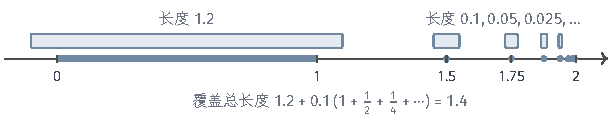
\includegraphics[width=103.7mm]{figures/02-abstract-mathematics/01-metric-and-measure/tikz/c2-outer-cover/figure.pdf}
  \caption{用可数个开区间覆盖集合$E=[0,1]\cup\{1.5,1.75,1.875,\dots\}$（深色）。浅色区间是一种覆盖：区间$(-0.1,1.1)$覆盖线段部分，长度依次减半的小区间覆盖离散的点。覆盖总长度为$1.2+0.1\cdot(1+\tfrac12+\tfrac14+\cdots)=1.4$；把各区间进一步缩短，总长度可以任意接近$1$，因此$\lambda^*(E)=1$。}
  \label{fig:measure-outer-cover}
\end{figure}

\paragraph{区间的外测度}
下界的困难在于覆盖可以有无限多个区间。闭区间的紧性把它化为有限覆盖，而有限覆盖可以沿实轴从左到右逐个检查。为了在第~\ref{sec:measure-stieltjes}小节复用，下面把长度换成单调函数的增量来叙述，取$F(x)=x$就回到长度。

\begin{lemma}[闭区间的有限开覆盖]
\label{lem:measure-finite-cover}
设$F:\mathbb R\to\mathbb R$单调不减，$a\le b$，开区间$(c_1,d_1),\dots,(c_m,d_m)$覆盖$[a,b]$。则
\[
 F(b)-F(a)\le\sum_{k=1}^m\bigl(F(d_k)-F(c_k)\bigr).
\]
\end{lemma}

\begin{proof}
对区间个数$m$归纳，同时对一切$a\le b$断言成立。点$b$落在某个区间中，不妨设$c_m<b<d_m$。若$c_m<a$，则$[a,b]\subseteq(c_m,d_m)$，由单调性$F(b)-F(a)\le F(d_m)-F(c_m)$，右边其余各项非负，结论成立。若$c_m\ge a$，则$[a,c_m]$中的点都不在$(c_m,d_m)$中，只能被其余$m-1$个区间覆盖；当$m=1$时这不可能，当$m\ge2$时由归纳假设，$F(c_m)-F(a)\le\sum_{k<m}(F(d_k)-F(c_k))$。再加上$F(d_m)-F(c_m)\ge F(b)-F(c_m)$，两式相加即得。
\end{proof}

\begin{lemma}[区间的Lebesgue外测度]
\label{lem:measure-interval-outer}
对任意区间$I$，$\lambda^*(I)=\ell(I)$；无界区间两边都为$+\infty$。
\end{lemma}

\begin{proof}
先看闭区间$[a,b]$。对任意$\varepsilon>0$，单个区间$(a-\varepsilon,b+\varepsilon)$覆盖它，所以$\lambda^*([a,b])\le b-a+2\varepsilon$。反过来，设开区间$(a_n,b_n)$覆盖$[a,b]$。有界闭区间是紧集（第~\ref{sec:metric-compactness}节的Heine--Borel判据），所以其中有限个，例如$n\le m$的那些，已经覆盖$[a,b]$。由引理~\ref{lem:measure-finite-cover}（取$F(x)=x$），$b-a\le\sum_{n\le m}(b_n-a_n)\le\sum_n(b_n-a_n)$。对一切覆盖取下确界，得$\lambda^*([a,b])\ge b-a$。

对端点为$a<b$的有界区间$I$，任取$0<\varepsilon<(b-a)/2$，有$[a+\varepsilon,b-\varepsilon]\subseteq I\subseteq[a,b]$，由单调性$b-a-2\varepsilon\le\lambda^*(I)\le b-a$，令$\varepsilon\to0$。无界区间包含任意长的闭区间，外测度为$+\infty$。
\end{proof}

\paragraph{区间满足Carathéodory判据}
只需对半直线验证，因为由定理~\ref{thm:measure-borel-generators}，它们生成$\mathcal B(\mathbb R)$。

\begin{lemma}[半直线的可测性]
\label{lem:measure-halfline-measurable}
对每个$a\in\mathbb R$，半直线$H=(a,+\infty)$是$\lambda^*$-Carathéodory可测的。
\end{lemma}

\begin{proof}
设$E\subseteq\mathbb R$，$\lambda^*(E)<+\infty$，任取$\varepsilon>0$，选开区间$I_n$覆盖$E$且$\sum_n\ell(I_n)\le\lambda^*(E)+\varepsilon$。每个$I_n$被点$a$分成两个区间$I_n\cap H$与$I_n\setminus H$（可能为空），长度之和等于$\ell(I_n)$。前者覆盖$E\cap H$，后者覆盖$E\setminus H$，由次可加性和引理~\ref{lem:measure-interval-outer}，
\[
 \begin{aligned}
  \lambda^*(E\cap H)+\lambda^*(E\setminus H)
  &\le\sum_n\ell(I_n\cap H)+\sum_n\ell(I_n\setminus H)\\
  &=\sum_n\ell(I_n)\le\lambda^*(E)+\varepsilon.
 \end{aligned}
\]
令$\varepsilon\to0$即得判据中的“$\ge$”。
\end{proof}

由Carathéodory定理，$\lambda^*$-可测集构成一个$\sigma$代数；它含全部半直线，从而含它们生成的$\mathcal B(\mathbb R)$。

\begin{definition}[Lebesgue测度]
\label{def:measure-lebesgue}
关于$\lambda^*$为Carathéodory可测的全体集合称为\term{Lebesgue可测集}（Lebesgue measurable set），记作$\mathcal L$；$\lambda^*$在$\mathcal L$上的限制$\lambda$称为实轴上的\term{Lebesgue测度}（Lebesgue measure）。$\lambda$在$\mathcal B(\mathbb R)$上的限制也称为Borel集上的Lebesgue测度，仍记作$\lambda$。
\end{definition}

综合以上结果，$(\mathbb R,\mathcal L,\lambda)$是完备测度空间，$\mathcal B(\mathbb R)\subseteq\mathcal L$，并且每个区间的Lebesgue测度等于它的长度。由于覆盖平移后仍是覆盖、长度不变，$\lambda^*(E+t)=\lambda^*(E)$对一切$t\in\mathbb R$成立，Lebesgue测度还具有平移不变性。

\paragraph{可数集的测度}
单点$\{x\}$被$(x-\varepsilon,x+\varepsilon)$覆盖，$\lambda(\{x\})\le2\varepsilon$，故为$0$。由可数次可加性，可数集的Lebesgue测度为$0$。回到第~\ref{sec:measure-jordan}小节的有理点集：$\lambda(\mathbb Q\cap[0,1])=0$，而$[0,1]$中的无理数集合测度为$\lambda([0,1])-0=1$。Jordan外测量把有理点算作$1$，是因为它只允许有限覆盖；可数覆盖把稠密而可数的集合正确地算作零。同时，$[0,1]$是不可数个单点之并，各单点测度为$0$，整体测度却为$1$，这兑现了第~\ref{sec:measure-null-sets}小节的说法：零测集的可数并仍是零测集，不可数并则不然。

\paragraph{Cantor集}
零测集是否一定可数？Cantor集给出否定的回答。

\begin{example}[Cantor集]
\label{ex:measure-cantor-set}
令$C_0=[0,1]$。把$C_{n-1}$中每个闭区间三等分，删去中间的开区间，得到$C_n$，它由$2^n$个长度为$3^{-n}$的闭区间组成，例如$C_1=[0,\tfrac13]\cup[\tfrac23,1]$，$C_2=[0,\tfrac19]\cup[\tfrac29,\tfrac13]\cup[\tfrac23,\tfrac79]\cup[\tfrac89,1]$。令$C=\bigcap_{n\ge0}C_n$，称为\term{Cantor集}（Cantor set）。它是闭集的交，是闭集，因而是Borel集。由$C\subseteq C_n$与有限可加性，
\[
 \lambda(C)\le\lambda(C_n)=2^n\cdot3^{-n}=(2/3)^n\to0,
\]
所以$\lambda(C)=0$。图~\ref{fig:measure-cantor-set}画出了前四步。
\end{example}

\begin{figure}[!htbp]
  \centering
  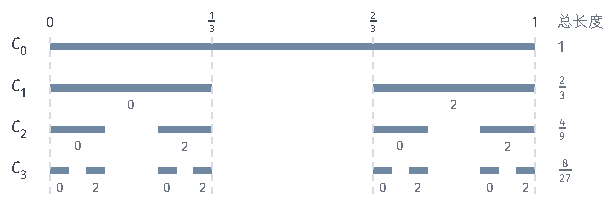
\includegraphics[width=104.1mm]{figures/02-abstract-mathematics/01-metric-and-measure/tikz/c2-cantor-set/figure.pdf}
  \caption{Cantor集构造的前四步。第$n$行$C_n$由$2^n$个长度为$3^{-n}$的闭区间组成，总长度$(2/3)^n$依次为$1,\tfrac23,\tfrac49,\tfrac{8}{27}$；区间下方的三进制数字$0$或$2$记录每一步选择左段还是右段。}
  \label{fig:measure-cantor-set}
\end{figure}

Cantor集虽然测度为零，却不可数。对每个$0$--$1$序列$s=(s_1,s_2,\dots)$，令$\phi(s)=\sum_{k\ge1}2s_k3^{-k}$，即三进制展开中只用数字$0$与$2$的数。按图~\ref{fig:measure-cantor-set}的读法，前$n$位数字决定了在每一步选左段（数字$0$）还是右段（数字$2$），对$n$归纳可知$\phi(s)$落在$C_n$的相应区间中，所以$\phi(s)\in C$。$\phi$是单射：若$s\ne t$且第一个不同的位置为$k$，不妨$s_k=1$、$t_k=0$，则
\[
 \phi(s)-\phi(t)\ge2\cdot3^{-k}-\sum_{j>k}2\cdot3^{-j}=2\cdot3^{-k}-3^{-k}=3^{-k}>0.
\]
全体$0$--$1$序列由对角线方法不可数，因此$C$不可数。可数集测度为零，但测度为零的集合不必可数；零测性度量的是集合占据的长度，基数度量的是元素的多少，二者不能互相推出。

\subsection{Lebesgue测度的逼近与推广}
\label{sec:measure-lebesgue-approximation}

\paragraph{开集外逼近与紧集内逼近}
Lebesgue测度是用开区间覆盖定义的，因此一个可测集合应当能被开集从外面逼近。取补集后，从里面也能用闭集乃至紧集逼近。这一性质把任意可测集合的测量问题化为开集和紧集这两类较好的集合，后面构造连续函数逼近和研究变量替换时都会用到。

\begin{theorem}[Lebesgue测度的正则性]
\label{thm:measure-lebesgue-regularity}
设$E\in\mathcal L$，$\varepsilon>0$。
\begin{enumerate}
 \item 存在开集$U\supseteq E$，使$\lambda(U\setminus E)<\varepsilon$。
 \item 存在闭集$F\subseteq E$，使$\lambda(E\setminus F)<\varepsilon$。
 \item 若$\lambda(E)<+\infty$，存在紧集$K\subseteq E$，使$\lambda(E\setminus K)<\varepsilon$。
\end{enumerate}
\end{theorem}

\begin{proof}
先对$\lambda(E)<+\infty$证明第1条。按$\lambda^*$的定义，存在开区间$I_n$覆盖$E$且$\sum_n\ell(I_n)<\lambda(E)+\varepsilon$。令$U=\bigcup_nI_n$，它是开集，$\lambda(U)\le\sum_n\ell(I_n)<\lambda(E)+\varepsilon$。由于$\lambda(E)$有限，$\lambda(U\setminus E)=\lambda(U)-\lambda(E)<\varepsilon$。一般情形把$E$切成有限测度的片$E_k=E\cap\{x:k-1\le|x|<k\}$，$k\ge1$，对每片取开集$U_k\supseteq E_k$使$\lambda(U_k\setminus E_k)<\varepsilon2^{-k}$；$U=\bigcup_kU_k$是开集，$U\setminus E\subseteq\bigcup_k(U_k\setminus E_k)$，故$\lambda(U\setminus E)<\varepsilon$。

对第2条，把第1条用于补集$\mathbb R\setminus E$，得开集$V\supseteq\mathbb R\setminus E$，$\lambda(V\setminus(\mathbb R\setminus E))<\varepsilon$。令$F=\mathbb R\setminus V$，它是闭集且$F\subseteq E$，而$E\setminus F=E\cap V=V\setminus(\mathbb R\setminus E)$，测度小于$\varepsilon$。

对第3条，先由第2条取闭集$F\subseteq E$使$\lambda(E\setminus F)<\varepsilon/2$。令$K_n=F\cap[-n,n]$，它有界闭，由Heine--Borel判据是紧集。集合$E\setminus K_n$递减，交为$E\setminus F$，且$\lambda(E\setminus K_1)\le\lambda(E)<+\infty$，由从上连续性$\lambda(E\setminus K_n)\to\lambda(E\setminus F)<\varepsilon/2$，所以$n$充分大时$K=K_n$满足要求。
\end{proof}

图~\ref{fig:measure-inner-outer-approx}以$E=[0,1]\setminus\{1/2\}$与$\varepsilon=0.25$为例：外侧开集$U=(-0.05,1.05)$包含$E$且多出的部分长度为$0.1$；内侧紧集$K=[0.05,0.45]\cup[0.55,0.95]$含于$E$，缺少的部分由四段长$0.05$的区间组成，总长度为$0.2$。两者都小于$\varepsilon$。这里逼近的是测度，而不是形状：$U\setminus E$与$E\setminus K$可以由多段组成，只要总长度小。

\begin{figure}[!htbp]
  \centering
  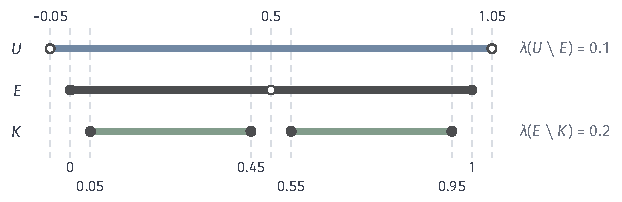
\includegraphics[width=105.3mm]{figures/02-abstract-mathematics/01-metric-and-measure/tikz/c2-inner-outer-approx/figure.pdf}
  \caption{可测集合$E=[0,1]\setminus\{1/2\}$的外开内紧逼近。中行是$E$，空心点表示被去掉的$1/2$；上行开集$U=(-0.05,1.05)\supseteq E$，$\lambda(U\setminus E)=0.1$；下行紧集$K=[0.05,0.45]\cup[0.55,0.95]\subseteq E$，$\lambda(E\setminus K)=0.2$。}
  \label{fig:measure-inner-outer-approx}
\end{figure}

\paragraph{Lebesgue可测集与Borel集}
正则性还说明，Lebesgue可测集与Borel集只差零测集。可数个开集的交是Borel集；对$E\in\mathcal L$，按第1条取开集$U_n\supseteq E$使$\lambda(U_n\setminus E)<1/n$，令$G=\bigcap_nU_n$，则$G\supseteq E$是Borel集，并且$\lambda(G\setminus E)\le\lambda(U_n\setminus E)<1/n$对一切$n$成立，故$\lambda(G\setminus E)=0$。

\begin{theorem}[Lebesgue测度是Borel测度的完备化]
\label{thm:measure-lebesgue-completion}
测度空间$(\mathbb R,\mathcal L,\lambda)$是Borel测度空间$(\mathbb R,\mathcal B(\mathbb R),\lambda)$的完备化：$E\in\mathcal L$当且仅当$E=B\cup M$，其中$B\in\mathcal B(\mathbb R)$，$M$包含于某个Borel零测集，并且此时$\lambda(E)=\lambda(B)$。
\end{theorem}

\begin{proof}
设$E\in\mathcal L$。由上一段，存在Borel集$G\supseteq E$，$\lambda(G\setminus E)=0$。对$\mathcal L$中的零测集$G\setminus E$再用一次上一段的结论，得Borel集$G'\supseteq G\setminus E$，$\lambda(G')=0$。于是$E=(G\setminus G')\cup(E\cap G')$，第一项是Borel集，第二项包含于Borel零测集$G'$，且$\lambda(E)=\lambda(G\setminus G')$。反过来，$\mathcal L$包含$\mathcal B(\mathbb R)$并且完备（定理~\ref{thm:measure-caratheodory-criterion}），所以每个$B\cup M$都属于$\mathcal L$，测度为$\lambda(B)$。
\end{proof}

由此可以区分三个范围：$\mathcal B(\mathbb R)\subseteq\mathcal L\subseteq\mathcal P(\mathbb R)$。两个包含都是严格的。Cantor集$C$测度为零，由完备性它的全部子集都Lebesgue可测，这样的子集比Borel集多，所以存在不是Borel集的Lebesgue可测集；这里的基数比较需要说明Borel集全体与$\mathbb R$等势，本章不展开。另一方面，借助选择公理可以构造不Lebesgue可测的集合（Vitali构造），我们只把它作为边界记住：并非所有子集都能被赋予与长度相容的测度，这正是测度只定义在$\sigma$代数上的原因。日常使用中，Borel集已经足够；需要“零测集的子集可测”时，再换用完备化。

\paragraph{多维Lebesgue测度}
在$\mathbb R^d$上，把区间换成开矩形$R=\prod_{i=1}^d(a_i,b_i)$（各边与坐标轴平行），长度换成体积$\prod_{i=1}^d(b_i-a_i)$，用可数个开矩形覆盖并对总体积取下确界，就得到外测度$\lambda_d^*$。上面的步骤逐一对应：闭矩形紧致，把可数覆盖化为有限覆盖后，用全部矩形的边坐标把一个大矩形切成网格，比较各网格小块的体积，可得闭矩形的外测度等于体积；把每个覆盖矩形沿超平面$\{\bm x:x_i=a\}$切成两个矩形，可得半空间$\{\bm x:x_i>a\}$满足Carathéodory判据；开集是可数个有理顶点开矩形之并，所以半空间生成$\mathcal B(\mathbb R^d)$。由此得到$\mathcal B(\mathbb R^d)$上体积的推广$\lambda_d$，称为$d$维Lebesgue测度，正则性与完备化的论证不变。$\lambda_d$与$d$个实轴Lebesgue测度的乘积在Borel集上相同，这一点需要乘积测度与唯一性定理，在第~\ref{sec:integral-iterated}节证明，那里也将区分乘积$\sigma$代数与其完备化。

\subsection{测度延拓的存在性和唯一性}
\label{sec:measure-extension}

\paragraph{从预测度延拓}
Lebesgue测度的构造可以抽象出来：先在一族简单集合上给出可数可加的赋值，再用覆盖得到外测度，最后由Carathéodory定理得到$\sigma$代数上的测度。这族简单集合只需对有限运算封闭。

\begin{definition}[集合代数与预测度]
\label{def:measure-algebra-premeasure}
$X$的一族子集$\mathcal R$若含$X$，并对补集和有限并封闭，称为$X$上的\term{集合代数}（algebra of sets）。$\mathcal R$上的映射$\mu_0:\mathcal R\to[0,+\infty]$若满足$\mu_0(\varnothing)=0$，并且对两两不交、并集仍属于$\mathcal R$的$A_1,A_2,\dots\in\mathcal R$有$\mu_0(\bigcup_nA_n)=\sum_n\mu_0(A_n)$，称为$\mathcal R$上的\term{预测度}（premeasure）。若存在$X_n\in\mathcal R$使$X=\bigcup_nX_n$且$\mu_0(X_n)<+\infty$，称$\mu_0$是$\sigma$有限的。
\end{definition}

集合代数只保证有限运算的结果仍在其中，可数并可能跑出去，所以预测度的可数可加性只在并集仍属于$\mathcal R$时提出。例如$\mathbb R$中有限个形如$(a,b]$（允许$a=-\infty$，$b=+\infty$时理解为$(a,+\infty)$）的不交区间之并构成集合代数，长度在其上是预测度；后一断言的证明与引理~\ref{lem:measure-interval-outer}的论证相同，在第~\ref{sec:measure-stieltjes}小节对一般单调函数给出。

\begin{theorem}[Carathéodory延拓定理]
\label{thm:measure-caratheodory}
设$\mu_0$是集合代数$\mathcal R$上的预测度，按引理~\ref{lem:measure-cover-outer}用$\mathcal R$中集合的可数覆盖定义外测度$\mu^*$。则$\mathcal R$中的集合都是$\mu^*$-Carathéodory可测的，且$\mu^*(A)=\mu_0(A)$对$A\in\mathcal R$成立。因此$\mu^*$限制在$\sigma(\mathcal R)$上是延拓$\mu_0$的测度。若$\mu_0$是$\sigma$有限的，$\sigma(\mathcal R)$上延拓$\mu_0$的测度是唯一的。
\end{theorem}

\begin{proof}
先证$\mu^*=\mu_0$在$\mathcal R$上成立。$A$本身覆盖$A$，故$\mu^*(A)\le\mu_0(A)$。设$C_n\in\mathcal R$覆盖$A$，令$D_n=A\cap C_n\setminus\bigcup_{k<n}C_k$。这些集合属于$\mathcal R$，两两不交，并集为$A\in\mathcal R$，由预测度的可数可加性与有限可加推出的单调性，$\mu_0(A)=\sum_n\mu_0(D_n)\le\sum_n\mu_0(C_n)$。对覆盖取下确界，得$\mu_0(A)\le\mu^*(A)$。

再证$A\in\mathcal R$满足Carathéodory判据。设$\mu^*(E)<+\infty$，$\varepsilon>0$，取$C_n\in\mathcal R$覆盖$E$且$\sum_n\mu_0(C_n)\le\mu^*(E)+\varepsilon$。$C_n\cap A$与$C_n\setminus A$属于$\mathcal R$，分别覆盖$E\cap A$与$E\setminus A$，并且$\mu_0(C_n)=\mu_0(C_n\cap A)+\mu_0(C_n\setminus A)$。于是
\[
 \begin{aligned}
  \mu^*(E\cap A)+\mu^*(E\setminus A)
  &\le\sum_n\mu_0(C_n\cap A)+\sum_n\mu_0(C_n\setminus A)\\
  &=\sum_n\mu_0(C_n)\le\mu^*(E)+\varepsilon.
 \end{aligned}
\]
由Carathéodory定理，可测集构成含$\mathcal R$的$\sigma$代数，所以含$\sigma(\mathcal R)$，$\mu^*$在其上是测度并延拓$\mu_0$。唯一性由下面的定理~\ref{thm:measure-uniqueness}给出：$\mathcal R$对有限交封闭，$\sigma$有限条件中的$X_n$正是那里要求的覆盖片。
\end{proof}

$\sigma$有限条件的作用是局部化：把全空间切成可数个有限质量的片，在每片上测度的总量有限，有限测度的唯一性论证可以逐片使用，最后由可数可加性拼回整体。

\paragraph{$\pi$系统与$\lambda$系统}
要说明两个测度在$\sigma(\mathcal C)$上相等，自然的做法是考察“两测度取值相等的集合”构成的族$\mathcal D$，希望它是含$\mathcal C$的$\sigma$代数。可是$\mathcal D$对补集和不交可数并封闭（由可数可加性），对一般的并却未必封闭，因为$\mu(A\cup B)=\mu(A)+\mu(B)-\mu(A\cap B)$要求先知道交集上的取值。这启发我们把封闭性要求拆成两部分。

\begin{definition}[$\pi$系统与$\lambda$系统]
\label{def:measure-pi-lambda-systems}
$X$的一族子集$\mathcal P$若对有限交封闭，称为\term{$\pi$系统}（pi-system）。一族子集$\mathcal D$若含$X$，对补集封闭，并对两两不交的可数并封闭，称为\term{$\lambda$系统}（lambda-system），也称\term{Dynkin系统}（Dynkin system）。
\end{definition}

$\sigma$代数既是$\pi$系统又是$\lambda$系统。反过来，若一族集合同时是二者，则它对有限交、补集封闭，从而对有限并封闭；对一般可数并，不交化$A_n\setminus\bigcup_{k<n}A_k=A_n\cap\bigcap_{k<n}(X\setminus A_k)$只用到有限交与补集，所以它是$\sigma$代数。

\begin{theorem}[$\pi$--$\lambda$定理]
\label{thm:measure-pi-lambda}
若$\pi$系统$\mathcal P$包含于$\lambda$系统$\mathcal D$，则$\sigma(\mathcal P)\subseteq\mathcal D$。
\end{theorem}

\begin{proof}
令$\ell(\mathcal P)$为所有包含$\mathcal P$的$\lambda$系统之交，它仍是$\lambda$系统，且$\ell(\mathcal P)\subseteq\mathcal D$。由上一段，只需证明$\ell(\mathcal P)$对有限交封闭，那时它是含$\mathcal P$的$\sigma$代数，于是$\sigma(\mathcal P)\subseteq\ell(\mathcal P)\subseteq\mathcal D$。

对集合$A$，令$\mathcal D_A=\{B:A\cap B\in\ell(\mathcal P)\}$。当$A\in\ell(\mathcal P)$时，$\mathcal D_A$是$\lambda$系统：$X\in\mathcal D_A$；若$B\in\mathcal D_A$，则$A\cap(X\setminus B)=X\setminus\bigl((X\setminus A)\cup(A\cap B)\bigr)$，括号内是$\ell(\mathcal P)$中两个不交集合之并，所以属于$\ell(\mathcal P)$，再取补集仍属于$\ell(\mathcal P)$；若$B_n\in\mathcal D_A$两两不交，则$A\cap\bigcup_nB_n=\bigcup_n(A\cap B_n)$是$\ell(\mathcal P)$中不交集合的可数并。

先取$A\in\mathcal P$。$\mathcal P$对交封闭，所以$\mathcal P\subseteq\mathcal D_A$，由最小性$\ell(\mathcal P)\subseteq\mathcal D_A$，即$A\cap B\in\ell(\mathcal P)$对一切$A\in\mathcal P$、$B\in\ell(\mathcal P)$成立。再任取$B\in\ell(\mathcal P)$，刚才的结论说明$\mathcal P\subseteq\mathcal D_B$，再由最小性$\ell(\mathcal P)\subseteq\mathcal D_B$。这就是说$\ell(\mathcal P)$对两个集合的交封闭。
\end{proof}

\paragraph{测度的唯一性}
有了$\pi$--$\lambda$定理，只需在生成$\pi$系统上比较两个测度。总量有限时，“取值相等的集合”构成$\lambda$系统；$\sigma$有限时，还需要一列共同的有限质量覆盖片。

\begin{theorem}[生成$\pi$系统上的唯一性]
\label{thm:measure-uniqueness}
设$\mathcal P$是$X$上的$\pi$系统，$\mu,\nu$是$(X,\sigma(\mathcal P))$上的测度，并在$\mathcal P$上取值相同。
\begin{enumerate}
 \item 若$\mu(X)=\nu(X)<+\infty$，则$\mu=\nu$。
 \item 若存在$X_1,X_2,\dots\in\mathcal P$，使$\bigcup_nX_n=X$且$\mu(X_n)=\nu(X_n)<+\infty$，则$\mu=\nu$。
\end{enumerate}
\end{theorem}

\begin{proof}
对第1条，令$\mathcal D=\{A\in\sigma(\mathcal P):\mu(A)=\nu(A)\}$。由假设$X\in\mathcal D$；若$A\in\mathcal D$，因两测度总量有限，$\mu(X\setminus A)=\mu(X)-\mu(A)=\nu(X)-\nu(A)=\nu(X\setminus A)$；不交可数并由可数可加性保持。所以$\mathcal D$是含$\mathcal P$的$\lambda$系统，由$\pi$--$\lambda$定理，$\mathcal D=\sigma(\mathcal P)$。

对第2条，固定$n$，令$\mu_n(A)=\mu(A\cap X_n)$、$\nu_n(A)=\nu(A\cap X_n)$。它们是有限测度，总量都等于$\mu(X_n)=\nu(X_n)$；对$A\in\mathcal P$，$A\cap X_n\in\mathcal P$，故$\mu_n(A)=\nu_n(A)$。由第1条，$\mu_n=\nu_n$。令$B_1=X_1$，$B_n=X_n\setminus\bigcup_{k<n}X_k\in\sigma(\mathcal P)$，它们两两不交，并为$X$，且$B_n\subseteq X_n$。对任意$A\in\sigma(\mathcal P)$，
\[
 \begin{aligned}
  \mu(A)&=\sum_n\mu(A\cap B_n)=\sum_n\mu_n(A\cap B_n)\\
  &=\sum_n\nu_n(A\cap B_n)=\sum_n\nu(A\cap B_n)=\nu(A).
 \end{aligned}
\]
\end{proof}

第2条要求覆盖片$X_n$取自$\mathcal P$，并且两测度在这些片上取有限的相同值；只知道“$\mu$与$\nu$各自$\sigma$有限”是不够的。在$\mathbb R$上取$\mathcal P=\{\varnothing\}\cup\{(a,b]:a<b\}$，令$\mu(A)=\#(A\cap\mathbb Q)$，$\nu=2\mu$。二者都是$\sigma$有限的：$\mathbb R$是可数个有理单点与零测集$\mathbb R\setminus\mathbb Q$之并。每个非退化区间$(a,b]$都含无限多个有理数，$\mu$、$\nu$在$\mathcal P$上都取$+\infty$（空集上都取$0$），但$\mu(\{0\})=1\ne2=\nu(\{0\})$。失败的原因是$\mathcal P$中没有有限质量的覆盖片。

对Lebesgue测度，取$\mathcal P$为$\varnothing$与全体$(a,b]$，覆盖片$X_n=(-n,n]$的长度有限，所以$\mathcal B(\mathbb R)$上满足$\lambda((a,b])=b-a$的测度只有一个。后面验证某个Borel测度等于$\lambda$或$\lambda$的倍数时，只需在区间上比较。

\subsection{Lebesgue--Stieltjes测度}
\label{sec:measure-stieltjes}

\paragraph{用单调函数的增量赋值}
长度给区间$(a,b]$赋值$b-a$，即函数$x\mapsto x$的增量。把它换成一般单调函数$F$的增量$F(b)-F(a)$，就改变了实轴上的累计规则：$F$增长快的地方质量多，$F$不变的地方没有质量，$F$跳跃的地方集中了点质量。这正是概率中分布函数描述分布的方式。

\begin{theorem}[Lebesgue--Stieltjes测度]
\label{thm:measure-stieltjes}
设$F:\mathbb R\to\mathbb R$单调不减且右连续。则$\mathcal B(\mathbb R)$上存在唯一的测度$\mu_F$，使
\[
 \mu_F((a,b])=F(b)-F(a),\qquad a<b.
\]
$\mu_F$称为$F$确定的\term{Lebesgue--Stieltjes测度}（Lebesgue--Stieltjes measure）。
\end{theorem}

\begin{proof}
记$F(+\infty)=\lim_{x\to+\infty}F(x)$与$F(-\infty)=\lim_{x\to-\infty}F(x)$，单调性保证极限在$[-\infty,+\infty]$中存在。在上一小节的集合代数$\mathcal R$（有限个不交区间$(a,b]$之并，$-\infty\le a<b\le+\infty$）上，令$\mu_0((a,b])=F(b)-F(a)$并对不交区间相加。与第~\ref{sec:measure-counting-length}小节相同，增量在共同细分上逐项相消，所以赋值与分割方式无关，且有限可加。

需要证明的是可数可加性：若$(a,b]$是不交区间$(a_n,b_n]$的可数并，则$F(b)-F(a)=\sum_n(F(b_n)-F(a_n))$。“$\ge$”方向：对任意$m$，前$m$个区间按左端点排序后互不相交地位于$(a,b]$中，增量之和不超过$F(b)-F(a)$，令$m\to\infty$。“$\le$”方向先设$a,b$有限。任取$\varepsilon>0$。由右连续性，取$a'\in(a,b)$使$F(a')-F(a)<\varepsilon$，取$b'_n>b_n$使$F(b'_n)-F(b_n)<\varepsilon2^{-n}$。开区间$(a_n,b'_n)$覆盖闭区间$[a',b]$，由紧性，有限个已经覆盖，由引理~\ref{lem:measure-finite-cover}，
\[
 F(b)-F(a')\le\sum_n\bigl(F(b'_n)-F(a_n)\bigr)\le\sum_n\bigl(F(b_n)-F(a_n)\bigr)+\varepsilon,
\]
从而$F(b)-F(a)\le\sum_n(F(b_n)-F(a_n))+2\varepsilon$。若$b=+\infty$或$a=-\infty$，对有限区间$(a,b]\cap(-M,M]$应用已证的结果（它是$(a_n,b_n]\cap(-M,M]$的不交并，各项增量不超过原增量），再令$M\to\infty$。

因此$\mu_0$是$\mathcal R$上的预测度，并且$\mu_0((-n,n])=F(n)-F(-n)<+\infty$，它是$\sigma$有限的。由Carathéodory延拓定理，$\mu_0$延拓为$\sigma(\mathcal R)=\mathcal B(\mathbb R)$上的唯一测度。
\end{proof}

右连续性在证明中用于把左端点从$a$挪到$a'$、把右端点从$b_n$挪到$b'_n$时只损失很小的增量。从测度一侧看，它是从上连续性的要求：$(a,b+1/n]$递减到$(a,b]$，测度从上连续给出$\mu_F((a,b])=\lim_nF(b+1/n)-F(a)$，这只有在$F$右连续时才等于$F(b)-F(a)$。

\paragraph{点质量与例子}
单点可写成递减交$\{x\}=\bigcap_n(x-1/n,x]$，首项测度有限，由从上连续性
\[
 \mu_F(\{x\})=\lim_{n\to\infty}\bigl(F(x)-F(x-1/n)\bigr)=F(x)-F(x-),
\]
其中$F(x-)$为左极限。所以$F$在$x$处的跳跃高度正是$x$处的点质量，$F$连续处没有点质量。取$F(x)=x$，$\mu_F$在区间上与长度一致，由唯一性就是Borel集上的Lebesgue测度$\lambda$。取阶跃函数$F=\mathbf 1_{[0,+\infty)}$，区间$(a,b]$含$0$时增量为$1$，否则为$0$，于是$\mu_F=\delta_0$。给$F$加上常数不改变任何增量，因而不改变$\mu_F$；只有增量才有意义。

\begin{example}[长度与点质量的混合]
\label{ex:measure-stieltjes-mixture}
令$F(x)=0$（$x<0$），$F(x)=x/2$（$0\le x<1$），$F(x)=1$（$x\ge1$）。$F$单调不减、右连续，在$x=1$处从$1/2$跳到$1$。于是$\mu_F(\{1\})=1/2$，而在$(0,1)$内$F$以斜率$1/2$增长。逐个比较区间上的取值可得$\mu_F=\tfrac12\lambda|_{[0,1]}+\tfrac12\delta_1$，例如
\[
 \mu_F((0.5,1])=F(1)-F(0.5)=1-0.25=0.75=\tfrac12\cdot0.5+\tfrac12.
\]
$\mu_F(\mathbb R)=F(+\infty)-F(-\infty)=1$，这是一个概率测度。图~\ref{fig:measure-stieltjes-jump}画出了$F$：斜坡部分的增量给出分布在区间上的质量，跳跃给出点质量。
\end{example}

\begin{figure}[!htbp]
  \centering
  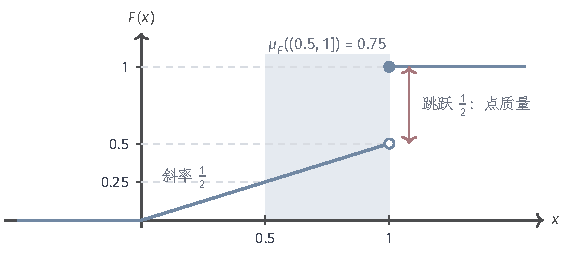
\includegraphics[width=96.5mm]{figures/02-abstract-mathematics/01-metric-and-measure/tikz/c2-stieltjes-jump/figure.pdf}
  \caption{右连续单调函数$F$确定的Lebesgue--Stieltjes测度。$F$在$[0,1)$上以斜率$1/2$增长，对应总量$1/2$、均匀分布在$[0,1]$上的质量；在$x=1$处跳跃$1/2$（实心点为$F(1)=1$，空心点为左极限$1/2$），对应点质量$\tfrac12\delta_1$。阴影竖条示意区间$(0.5,1]$的测度$F(1)-F(0.5)=0.75$。}
  \label{fig:measure-stieltjes-jump}
\end{figure}

连续的$F$不产生点质量，但这不意味着$\mu_F$一定像长度那样“摊开”分布。第~\ref{sec:measure-decomposition}节将用Cantor集构造一个连续的$F$，它的测度集中在零测的Cantor集上；至于$\mu_F$何时能表示成相对于长度的密度，留到第~\ref{chap:densities-change-of-measure}章回答。

\section{可测映射与可测函数}
\label{sec:measure-measurable-maps}

有了测度，我们还要处理定义在可测空间上的映射：随机实验的结果被读成一个数，平面上的点被投影到坐标轴，一列函数取逐点极限。每当对映射的输出提出“是否落在某集合中”的问题，就需要输入端能够测量相应的点集。本节用原像刻画这一要求，先给出一般可测映射的判据与复合规则，再专门研究实值可测函数，证明常见运算与可数极限保持可测性。用简单函数逼近一般可测函数的构造，留到第~\ref{chap:integration}章定义积分时展开。

\subsection{原像判据与可测复合}
\label{sec:measure-preimage-criterion}

\paragraph{可测映射的定义}
对映射$f:X\to Y$与$B\subseteq Y$，原像$f^{-1}(B)=\{x\in X:f(x)\in B\}$是“输出落在$B$中”的那些输入。原像记号对任意映射都有意义，并不要求$f$可逆（可参考\BookChapterRef{chap:sets-relations-maps}{卷一“集合、关系与映射”章}）。若输出端能提出的每个集合问题，在输入端都对应一个可测集合，就说$f$是可测的。

\begin{definition}[可测映射]
\label{def:measure-measurable-map}
设$(X,\mathcal A)$、$(Y,\mathcal B)$是可测空间。若对每个$B\in\mathcal B$都有$f^{-1}(B)\in\mathcal A$，称映射$f:X\to Y$为$\mathcal A/\mathcal B$-\term{可测映射}（measurable map），简称可测。
\end{definition}

可测性同时取决于两端的$\sigma$代数。在$X=\{1,2,3,4\}$上取由$\varnothing$、$\{1,2\}$、$\{3,4\}$、$X$组成的$\sigma$代数$\mathcal A$，在$Y=\{a,b\}$上取$\mathcal P(Y)$。令$f(1)=f(2)=a$、$f(3)=f(4)=b$，则$f^{-1}(\{a\})=\{1,2\}$、$f^{-1}(\{b\})=\{3,4\}$都可测，$f$可测。令$g(1)=a$、$g(2)=g(3)=g(4)=b$，则$g^{-1}(\{a\})=\{1\}\notin\mathcal A$，$g$不可测：输入端只知道点属于哪一组，无法回答“输出是否为$a$”。若把$Y$上的$\sigma$代数换成$\{\varnothing,Y\}$，$g$又变成可测的，因为输出端不再提出任何非平凡问题。

\paragraph{生成族判据}
直接检查$\mathcal B$中的每个集合往往不可行，例如$\mathcal B(\mathbb R)$中的集合无法逐一列出。原像与集合运算可交换，这使我们只需检查生成族。

\begin{lemma}[生成族判据]
\label{lem:measure-generator-criterion}
设$\mathcal B=\sigma(\mathcal C)$。若对每个$C\in\mathcal C$都有$f^{-1}(C)\in\mathcal A$，则$f$是$\mathcal A/\mathcal B$可测的。
\end{lemma}

\begin{proof}
令$\mathcal E=\{B\subseteq Y:f^{-1}(B)\in\mathcal A\}$。由$f^{-1}(Y)=X$、$f^{-1}(Y\setminus B)=X\setminus f^{-1}(B)$与$f^{-1}(\bigcup_nB_n)=\bigcup_nf^{-1}(B_n)$，$\mathcal E$是$Y$上的$\sigma$代数。它含$\mathcal C$，所以含$\sigma(\mathcal C)=\mathcal B$。
\end{proof}

图~\ref{fig:measure-preimage-criterion}示意了这一判据：只要生成族中每个集合的原像都落在$\mathcal A$中，由补集与可数并生成的其余集合，其原像也由相应运算得到，自动落在$\mathcal A$中。

\begin{figure}[!htbp]
  \centering
  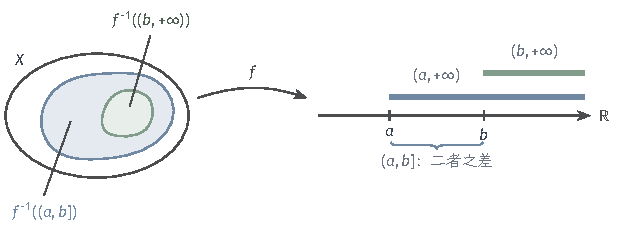
\includegraphics[width=105.1mm]{figures/02-abstract-mathematics/01-metric-and-measure/tikz/c2-preimage-criterion/figure.pdf}
  \caption{原像判据。右侧是输出空间$\mathbb R$中的生成集合$(a,+\infty)$与$(b,+\infty)$，左侧是它们在输入空间$X$中的原像。原像保持集合运算：$(a,b]=(a,+\infty)\setminus(b,+\infty)$的原像等于两个原像之差，所以只要生成集合的原像可测，由它们运算得到的集合，原像也可测。}
  \label{fig:measure-preimage-criterion}
\end{figure}

\paragraph{复合与连续映射}
若$f:(X,\mathcal A)\to(Y,\mathcal B)$与$g:(Y,\mathcal B)\to(Z,\mathcal C)$都可测，则对$C\in\mathcal C$，
\[
 (g\circ f)^{-1}(C)=f^{-1}\bigl(g^{-1}(C)\bigr),
\]
其中$g^{-1}(C)\in\mathcal B$，再由$f$可测得$f^{-1}(g^{-1}(C))\in\mathcal A$，所以复合$g\circ f$可测。这里要求中间空间$Y$上两次使用的是同一个$\sigma$代数$\mathcal B$。

设$(X,d_X)$、$(Y,d_Y)$是度量空间，$f$连续。由第~\ref{sec:metric-continuous-maps}节，开集的原像是开集，因而属于$\mathcal B(X)$；开集生成$\mathcal B(Y)$，由引理~\ref{lem:measure-generator-criterion}，$f$是$\mathcal B(X)/\mathcal B(Y)$可测的。这个结论依赖两端都取Borel结构。若把两端都换成Lebesgue可测集$\mathcal L$，连续函数$f:\mathbb R\to\mathbb R$未必$\mathcal L/\mathcal L$可测：可以构造连续严格单调的函数$f$与Lebesgue零测集的子集$S$（由完备性，$S\in\mathcal L$），使$f^{-1}(S)$不是Lebesgue可测集。这里不展开构造，只记住：可测性必须写清两端的集合族，不能把目标端的Borel结构随意换成某个测度的完备化。

\subsection{可测函数的运算}
\label{sec:measure-function-operations}

\paragraph{阈值判据}
最常用的可测映射是取实数值的函数。目标端取$\mathcal B(\mathbb R)$，由定理~\ref{thm:measure-borel-generators}，半直线$(a,+\infty)$生成它，判据化为检查阈值集合。

\begin{definition}[可测函数]
\label{def:measure-measurable-function}
设$(X,\mathcal A)$是可测空间。若$f:X\to\mathbb R$是$\mathcal A/\mathcal B(\mathbb R)$可测的，称$f$为\term{可测函数}（measurable function）。对取值于扩展实数$[-\infty,+\infty]$的函数，若对每个$a\in\mathbb R$都有$\{f>a\}=\{x:f(x)>a\}\in\mathcal A$，也称它可测。当$(X,\mathcal A)=(\mathbb R^d,\mathcal B(\mathbb R^d))$时，称为\term{Borel可测函数}（Borel measurable function）。
\end{definition}

\begin{lemma}[阈值判据]
\label{lem:measure-threshold}
$f:X\to\mathbb R$可测，当且仅当对每个有理数$a$，$\{f>a\}\in\mathcal A$。
\end{lemma}

\begin{proof}
必要性：$\{f>a\}=f^{-1}((a,+\infty))$。充分性：由定理~\ref{thm:measure-borel-generators}，有理端点半直线$(a,+\infty)$生成$\mathcal B(\mathbb R)$，再用引理~\ref{lem:measure-generator-criterion}。
\end{proof}

用补集与可数运算还可得到其他阈值集合，例如$\{f\ge a\}=\bigcap_n\{f>a-1/n\}$、$\{f\le a\}=X\setminus\{f>a\}$，它们也都可测。

\paragraph{示性函数与简单函数}
集合可测性与函数可测性通过指示函数相连。对$A\subseteq X$，$\{\mathbf 1_A>a\}$在$a<0$时为$X$，在$0\le a<1$时为$A$，在$a\ge1$时为$\varnothing$，所以$\mathbf 1_A$可测当且仅当$A\in\mathcal A$。例如$\mathbf 1_{\mathbb Q}$在$(\mathbb R,\mathcal B(\mathbb R))$上可测，因为$\mathbb Q$是Borel集；第~\ref{sec:measure-jordan}小节中它对应的集合连Jordan可测都不是，测度论却可以直接处理它。

\begin{definition}[简单函数]
\label{def:measure-simple-function}
只取有限多个实数值的可测函数称为\term{简单函数}（simple function）。
\end{definition}

设简单函数$\varphi$的不同取值为$c_1,\dots,c_m$，令$A_i=\varphi^{-1}(\{c_i\})$，它们是可测集合，两两不交，并为$X$，于是
\[
 \varphi=\sum_{i=1}^mc_i\mathbf 1_{A_i}.
\]
反过来，任意可测集合$B_j$的有限线性组合$\sum_jb_j\mathbf 1_{B_j}$只取有限多个值，每个取值集合都是若干$B_j$及其补集的交之并，因此是简单函数。同一个简单函数可以有多种写法，例如$\mathbf 1_{[0,2]}=\mathbf 1_{[0,1]}+\mathbf 1_{(1,2]}$；按不同取值写出的上式是标准写法。第~\ref{chap:integration}章将先对简单函数定义积分，再用简单函数逼近一般可测函数。

\paragraph{代数运算}
可测函数经过加、乘、取绝对值等运算后仍然可测。困难在于和的阈值集合$\{f+g>a\}$不能直接写成$f$与$g$各自阈值集合的有限组合，需要用有理数作可数分拆。

\begin{theorem}[可测函数的运算]
\label{thm:measure-function-operations}
设$f,g:X\to\mathbb R$可测，$c\in\mathbb R$，$\varphi:\mathbb R\to\mathbb R$连续。则$cf$、$f+g$、$\varphi\circ f$、$fg$、$|f|$、$\max\{f,g\}$、$\min\{f,g\}$都可测；若$g$处处不为零，$f/g$也可测。
\end{theorem}

\begin{proof}
$\varphi\circ f$是可测映射与Borel可测的连续映射之复合，由上一小节可测。取$\varphi(t)=ct$与$\varphi(t)=|t|$，得$cf$与$|f|$可测；取$\varphi(t)=t^2$，得$f^2$可测。

对和，若$f(x)+g(x)>a$，则$f(x)>a-g(x)$，在两者之间取有理数$q$，有$f(x)>q$且$g(x)>a-q$；反之这两式蕴含$f(x)+g(x)>a$。所以
\[
 \{f+g>a\}=\bigcup_{q\in\mathbb Q}\bigl(\{f>q\}\cap\{g>a-q\}\bigr),
\]
是可数个可测集合之并。于是$f-g=f+(-1)g$也可测。积由恒等式$fg=\tfrac14\bigl((f+g)^2-(f-g)^2\bigr)$得到，最大值与最小值由$\max\{f,g\}=\tfrac12(f+g+|f-g|)$与$\min\{f,g\}=\tfrac12(f+g-|f-g|)$得到。若$g$处处非零，$g$是到$\mathbb R\setminus\{0\}$的可测映射，$t\mapsto1/t$在$\mathbb R\setminus\{0\}$上连续，所以$1/g$可测，$f/g=f\cdot(1/g)$可测。
\end{proof}

允许取扩展实数值时，运算本身可能无定义。$f+g$在$f(x)=+\infty$、$g(x)=-\infty$的点没有意义，必须先说明这样的点不出现，或者在那里另作约定；乘积还要约定$0\cdot(\pm\infty)$。只有在这些点上的值被确定以后，才能谈论运算结果是否可测，不能把形式上的式子当作已经定义好的函数。

\subsection{函数列的可测性}
\label{sec:measure-function-sequences}

\paragraph{可数极限}
分析中的许多函数是作为函数列的极限得到的，例如级数的和与逐次逼近的结果。下面的定理说明，可数个可测函数取上确界、下确界和极限后仍然可测。

\begin{theorem}[可数极限的可测性]
\label{thm:measure-limits}
设$f_1,f_2,\dots:X\to[-\infty,+\infty]$可测。则$\sup_nf_n$、$\inf_nf_n$、$\limsup_nf_n$、$\liminf_nf_n$可测。若对每个$x$，极限$\lim_nf_n(x)$在$[-\infty,+\infty]$中存在，则极限函数可测。
\end{theorem}

\begin{proof}
$\sup_nf_n(x)>a$当且仅当某个$f_n(x)>a$，所以$\{\sup_nf_n>a\}=\bigcup_n\{f_n>a\}$可测。对下确界，$\{\inf_nf_n\ge a\}=\bigcap_n\{f_n\ge a\}$可测，从而$\{\inf_nf_n>a\}=\bigcup_k\{\inf_nf_n\ge a+1/k\}$可测。上极限与下极限是可数次上、下确界的组合：
\[
 \limsup_{n\to\infty}f_n=\inf_{n\ge1}\sup_{k\ge n}f_k,\qquad \liminf_{n\to\infty}f_n=\sup_{n\ge1}\inf_{k\ge n}f_k,
\]
由前两步可测。极限存在时它等于上极限，因而可测。
\end{proof}

这个定理只保证极限对象是可测函数，可以对它提出测度与积分的问题；它并没有说极限函数的积分等于积分的极限。这种交换需要另外的条件，是第~\ref{chap:integration}章收敛定理的内容。

\paragraph{零测修改}
函数在零测集上的取值通常无关紧要，但修改后的函数是否仍然可测，取决于测度空间是否完备。设$f$可测，$g$与$f$仅在某个零测集$N$内的点上可能不同。若空间完备，则
\[
 \{g>a\}=\bigl(\{f>a\}\setminus N\bigr)\cup\bigl(\{g>a\}\cap N\bigr),
\]
第一项可测，第二项是零测集的子集，由完备性可测，所以$g$可测。若空间不完备，结论可能失败：在第~\ref{sec:measure-null-sets}小节的例子中，$X=\{1,2,3\}$，$\mathcal A=\{\varnothing,\{1\},\{2,3\},X\}$，$\mu=\delta_1$，取$f=0$、$g=\mathbf 1_{\{2\}}$，二者只在零测集$\{2,3\}$内不同，但$\{g>0\}=\{2\}$不可测。因此在一般测度空间中说“$g$与$f$几乎处处相等”时，要么先确认$g$可测，要么选取一个可测的代表，或者换到完备化空间上讨论。

\paragraph{不可数运算的边界}
可数性在上面的证明中不可缺少。设$S\subseteq\mathbb R$不是Borel集（这样的集合存在，例如上一节提到的不Lebesgue可测的集合）。对每个$s\in S$，$f_s=\mathbf 1_{\{s\}}$是Borel可测函数，但它们的逐点上确界
\[
 \sup_{s\in S}f_s=\mathbf 1_S
\]
不是Borel可测函数，因为$\{\mathbf 1_S>0\}=S$。证明中$\{\sup f_n>a\}=\bigcup_n\{f_n>a\}$只在指标可数时才是$\sigma$代数允许的运算；指标不可数时，同样的式子给出的是不可数并，可测性无从保证。

\section{推前测度}
\label{sec:measure-pushforward}

可测映射保证输出端的集合问题在输入端有意义。若输入端还配有测度，就可以回答“输出落在$B$中的质量有多少”：把会被送进$B$的输入全部找出来，累计它们的质量。本节用这一想法定义推前测度，核对它的可加性、复合与总量的变化，再用多对一映射和坐标投影计算具体的推前。整节只用到原像与测度的取值；推前测度下的积分换元公式在第~\ref{sec:integral-change-of-variables}节建立。

\subsection{推前测度的定义与性质}
\label{sec:measure-pushforward-def}

\paragraph{用原像累计质量}
设$T:(X,\mathcal A)\to(Y,\mathcal B)$可测，$\mu$是$(X,\mathcal A)$上的测度。对$B\in\mathcal B$，输出落在$B$中的输入恰是$T^{-1}(B)$，它可测，于是可以取它的质量作为$B$的质量。

\begin{definition}[推前测度]
\label{def:measure-pushforward}
设$T:(X,\mathcal A)\to(Y,\mathcal B)$可测，$\mu$是$(X,\mathcal A)$上的测度。令
\[
 (T_\#\mu)(B)=\mu\bigl(T^{-1}(B)\bigr),\qquad B\in\mathcal B,
\]
称$T_\#\mu$为$\mu$在$T$下的\term{推前测度}（pushforward measure）。
\end{definition}

\begin{theorem}[推前测度的基本性质]
\label{thm:measure-pushforward-properties}
在上述记号下：
\begin{enumerate}
 \item $T_\#\mu$是$(Y,\mathcal B)$上的测度，且$(T_\#\mu)(Y)=\mu(X)$；特别地，有限测度推前后仍有限，概率测度推前后仍是概率测度。
 \item 若$S:(Y,\mathcal B)\to(Z,\mathcal C)$也可测，则$(S\circ T)_\#\mu=S_\#(T_\#\mu)$。
\end{enumerate}
\end{theorem}

\begin{proof}
对第1条，$T^{-1}(\varnothing)=\varnothing$给出空集为零。若$B_n\in\mathcal B$两两不交，则它们的原像也两两不交：一个$x$若同时属于$T^{-1}(B_n)$与$T^{-1}(B_m)$，$T(x)$就同时属于$B_n$与$B_m$。由$T^{-1}(\bigcup_nB_n)=\bigcup_nT^{-1}(B_n)$和$\mu$的可数可加性，
\[
 (T_\#\mu)\Bigl(\bigcup_nB_n\Bigr)=\mu\Bigl(\bigcup_nT^{-1}(B_n)\Bigr)=\sum_n\mu\bigl(T^{-1}(B_n)\bigr)=\sum_n(T_\#\mu)(B_n).
\]
总量由$T^{-1}(Y)=X$得到。对第2条，$S\circ T$可测（第~\ref{sec:measure-preimage-criterion}小节），且对$C\in\mathcal C$，$(S\circ T)^{-1}(C)=T^{-1}(S^{-1}(C))$，于是$((S\circ T)_\#\mu)(C)=\mu(T^{-1}(S^{-1}(C)))=(T_\#\mu)(S^{-1}(C))=(S_\#(T_\#\mu))(C)$。
\end{proof}

第2条说明，分两步传递质量与一步传递质量的结果相同；这使我们可以把复杂的映射拆成简单映射逐步计算推前。

\paragraph{保持测度的映射}
当$T$把空间映到自身时，可以问质量分布是否在传递后保持不变。若可测映射$T:(X,\mathcal A)\to(X,\mathcal A)$满足$T_\#\mu=\mu$，即$\mu(T^{-1}(A))=\mu(A)$对一切$A\in\mathcal A$成立，称$T$\term{保持测度}（measure-preserving）。在$X=\{0,1,\dots,n-1\}$上取计数测度与循环移位$T(k)=k+1\bmod n$，$T$是双射，$T^{-1}(A)$与$A$元素个数相同，所以$T$保持计数测度。在实轴上，平移$T(x)=x+t$满足$T^{-1}(B)=B-t$，由Lebesgue测度的平移不变性，$\lambda(B-t)=\lambda(B)$，平移保持$\lambda$。

伸缩则改变长度。令$T(x)=2x$。区间$(a,b]$的原像是$T^{-1}((a,b])=(a/2,b/2]$，所以$(T_\#\lambda)((a,b])=(b-a)/2$。两个测度$T_\#\lambda$与$\tfrac12\lambda$在$\pi$系统$\{\varnothing\}\cup\{(a,b]\}$上一致，且在覆盖片$(-n,n]$上都取有限值$n$，由定理~\ref{thm:measure-uniqueness}，$T_\#\lambda=\tfrac12\lambda$。把实轴拉长一倍，同一个输出区间只收集到原来一半长度的输入。

\paragraph{$\sigma$有限性一般不保持}
总量在推前下不变，因此有限与概率的性质保持；$\sigma$有限性却可能丢失，因为推前可以把无限多片有限质量集中到一个点。在$\mathbb N$上取计数测度$\mu$，它是$\sigma$有限的。令$T$把$\mathbb N$映到单点集$Y=\{y\}$（取$\mathcal P(Y)$），则$(T_\#\mu)(\{y\})=\mu(\mathbb N)=+\infty$；$Y$的可测子集只有$\varnothing$与$\{y\}$，无法写成有限质量集合的可数并，$T_\#\mu$不是$\sigma$有限的。需要唯一性定理或后面的分解定理时，推前测度的$\sigma$有限性必须单独核对。

\subsection{合并与投影产生的测度}
\label{sec:measure-merge-projection}

\paragraph{多对一映射合并质量}
推前不要求$T$是单射。若有几个输入被送到同一个输出，它们的质量在输出处相加。设$X=\{1,2,3,4\}$上的测度$\mu$给四个点分别赋权$0.1,0.2,0.3,0.4$，$T(1)=T(3)=a$，$T(2)=T(4)=b$。则$T^{-1}(\{a\})=\{1,3\}$，$T^{-1}(\{b\})=\{2,4\}$，
\[
 T_\#\mu=0.4\,\delta_a+0.6\,\delta_b.
\]
图~\ref{fig:measure-pushforward-merge}(a)画出了这一过程：每个输出点收集其全部原像的权重，原来的四个点在输出端只剩两个，总量仍为$1$。

推前还可以把分布在区间上的质量合并成点质量。令$\mu=\lambda|_{[0,1]}$，$T$为取常值$c$的映射。对Borel集$B$，若$c\in B$，则$T^{-1}(B)=\mathbb R$，否则$T^{-1}(B)=\varnothing$，所以$(T_\#\mu)(B)=\mathbf 1_B(c)\cdot\lambda([0,1])$，即$T_\#\mu=\delta_c$。每个单点在$\mu$下质量为零，推前后却得到质量为$1$的点；区别在于原像$T^{-1}(\{c\})$是整个区间，而不是单点。若改用$T(x)=\lfloor2x\rfloor$，原像$T^{-1}(\{0\})\cap[0,1]=[0,\tfrac12)$、$T^{-1}(\{1\})\cap[0,1]=[\tfrac12,1)$、$T^{-1}(\{2\})\cap[0,1]=\{1\}$，得$T_\#\mu=\tfrac12\delta_0+\tfrac12\delta_1$，见图~\ref{fig:measure-pushforward-merge}(b)。

\begin{figure}[!htbp]
  \centering
  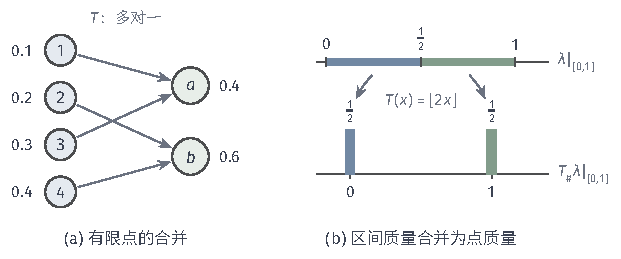
\includegraphics[width=105.1mm]{figures/02-abstract-mathematics/01-metric-and-measure/tikz/c2-pushforward-merge/figure.pdf}
  \caption{推前测度累计原像的质量。(a)四个带权点经多对一映射送到$a,b$两点，$a$收集点$1,3$的权重$0.1+0.3=0.4$，$b$收集点$2,4$的权重$0.2+0.4=0.6$；(b)$[0,1]$上的长度测度经$T(x)=\lfloor2x\rfloor$推前，原像$[0,\tfrac12)$与$[\tfrac12,1)$的长度分别汇集为点$0$和点$1$处的质量$\tfrac12$，单点$\{1\}$的长度为零，不贡献质量。}
  \label{fig:measure-pushforward-merge}
\end{figure}

\paragraph{坐标投影与边缘测度}
多元问题中最常见的多对一映射是坐标投影。设$\mu$是$\mathcal B(\mathbb R^d)$上的测度，$1\le k<d$，$\pi(\bm x)=(x_1,\dots,x_k)$。$\pi$连续，因而Borel可测，且对$B\in\mathcal B(\mathbb R^k)$有$\pi^{-1}(B)=B\times\mathbb R^{d-k}$，所以
\[
 (\pi_\#\mu)(B)=\mu\bigl(B\times\mathbb R^{d-k}\bigr).
\]
$\pi_\#\mu$称为$\mu$在前$k$个坐标上的\term{边缘测度}（marginal measure）：它忽略后$d-k$个坐标，只记录前$k$个坐标落在何处。卷一用联合分布对其余变量求和或积分得到边缘分布（可参考\BookChapterRef{chap:random-vectors}{卷一“随机向量与联合分布”章}），这里的定义只用集合原像，对离散与连续情形同样适用。

\begin{example}[点质量与单位正方形的投影]
\label{ex:measure-projection-marginal}
在$\mathbb R^2$上取$\mu=0.2\,\delta_{(0,0)}+0.3\,\delta_{(0,1)}+0.5\,\delta_{(1,1)}$。第一坐标的投影$\pi_1$把$(0,0)$与$(0,1)$都送到$0$，所以$(\pi_1)_\#\mu=0.5\,\delta_0+0.5\,\delta_1$；第二坐标的投影把$(0,1)$与$(1,1)$都送到$1$，所以$(\pi_2)_\#\mu=0.2\,\delta_0+0.8\,\delta_1$。

再取$\nu=\lambda_2|_{[0,1]^2}$。对$B=(a,b]$，$\pi_1^{-1}(B)\cap[0,1]^2=\bigl((a,b]\cap[0,1]\bigr)\times[0,1]$是一个矩形，面积等于$\lambda((a,b]\cap[0,1])$乘以$1$。于是$(\pi_1)_\#\nu$与$\lambda|_{[0,1]}$在全部$(a,b]$上一致，总量都为$1$，由定理~\ref{thm:measure-uniqueness}，二者在$\mathcal B(\mathbb R)$上相等。图~\ref{fig:measure-projection-marginal}画出了两种情形。
\end{example}

\begin{figure}[!htbp]
  \centering
  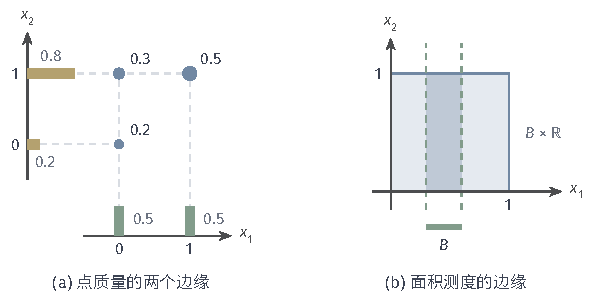
\includegraphics[width=100.9mm]{figures/02-abstract-mathematics/01-metric-and-measure/tikz/c2-projection-marginal/figure.pdf}
  \caption{坐标投影产生的边缘测度。(a)平面上三个点质量$0.2,0.3,0.5$，向横轴投影得到$0.5\delta_0+0.5\delta_1$，向纵轴投影得到$0.2\delta_0+0.8\delta_1$；(b)单位正方形上的面积测度，横轴区间$B$的边缘质量等于竖条$B\times\mathbb R$与正方形之交的面积，结果是$[0,1]$上的长度。}
  \label{fig:measure-projection-marginal}
\end{figure}

边缘测度的总量与原测度相同，但$\sigma$有限性同样可能丢失：对整个平面上的$\lambda_2$，任一非退化区间$B$都有$(\pi_1)_\#\lambda_2(B)=\lambda_2(B\times\mathbb R)=+\infty$，输出测度在每个非空开区间上都无限。对坐标积分把联合测度的计算化为边缘上的计算，以及一般推前测度下的积分公式，都在第~\ref{chap:integration}章建立；边缘测度何时有密度、密度怎样计算，在第~\ref{chap:densities-change-of-measure}章讨论。这里不预设输出测度一定有密度：上面的点质量例子中，边缘测度就是离散的。

\section{测度之间的关系}
\label{sec:measure-relations}

前面几节在同一个可测空间上放过多种测度：长度、点质量、计数、加权和，以及由映射推前得到的输出测度。同一族可测集合可以被不同的规则赋值，于是自然要问两种赋值之间有什么关系。本节固定可测空间$(X,\mathcal A)$及其上的两个非负测度$\mu,\nu$，只回答两个最粗的问题：一种测度忽略的集合，另一种是否也忽略；两种质量能否分别集中在互不相交的区域。两个问题都只读取集合上的质量，不需要积分，也不需要任何密度。

\subsection{绝对连续与等价测度}
\label{sec:measure-absolute-continuity}

第~\ref{sec:measure-spaces-def}节说过，“可以忽略”总是相对于某个测度而言的。比较两个测度时，最基本的信息就是它们的零测集族怎样相互包含。

\paragraph{零测集的包含关系}
设想$\mu$是我们用来判断“哪些事件可以忽略”的参考测度。若凡是$\mu$忽略的集合，$\nu$也一律忽略，那么在$\mu$下几乎处处成立的结论，在$\nu$下也几乎处处成立。这个单向要求就是绝对连续。

\begin{definition}[绝对连续与等价测度]
\label{def:measure-absolutely-continuous}
设$\mu,\nu$是可测空间$(X,\mathcal A)$上的非负测度。若对每个$A\in\mathcal A$，
\[
 \mu(A)=0\ \Longrightarrow\ \nu(A)=0,
\]
就称$\nu$相对于$\mu$\term{绝对连续}（absolutely continuous），记作$\nu\ll\mu$。若$\nu\ll\mu$与$\mu\ll\nu$同时成立，就称$\mu$与$\nu$是\term{等价测度}（equivalent measures），记作$\mu\sim\nu$。
\end{definition}

记号的方向需要留意：$\nu\ll\mu$说的是$\mu$的零测集族包含在$\nu$的零测集族之中，参考测度$\mu$写在右边。定义只比较“是否为零”，不比较非零质量的大小。

\begin{example}[两点空间上的单向关系]
取$X=\{0,1\}$，$\mathcal A$为全部子集，$\mu=\delta_0+\delta_1$，$\nu=\delta_0$。$\mu$给每个单点质量$1$，所以$\mu$的零测集只有空集，条件“$\mu(A)=0\Rightarrow\nu(A)=0$”只需对$A=\varnothing$检查，$\nu\ll\mu$成立。反方向不成立：$\nu(\{1\})=0$，而$\mu(\{1\})=1$。这里$\nu$在点$1$的权重为零，$\mu$却认为这一点有质量；图~\ref{fig:measure-absolute-continuity}(a)中右侧那根缺失的绿色柱就是这一反例。

再取$\rho=2\delta_0+5\delta_1$。$\rho$与$\mu$的零测集都只有空集，于是$\rho\sim\mu$；但$\rho(\{1\})=5\ne1=\mu(\{1\})$。等价只说明两种测度认可同一族零测集，不说明它们给同一集合的质量相同。
\end{example}

\paragraph{只检查单点为什么不够}
在实轴上，单点、可数集通常是Lebesgue零测集，人们容易只拿单点来检验绝对连续。$\delta_0$相对于$\lambda$不绝对连续，这确实可以由单点看出：$\lambda(\{0\})=0$，而$\delta_0(\{0\})=1$。但单点检查一般不够。记$\lambda|_{[0,1]}(A)=\lambda(A\cap[0,1])$、$\lambda|_{[2,3]}(A)=\lambda(A\cap[2,3])$，它们是第~\ref{sec:measure-spaces-def}节中限制到可测子集所得的测度，这里看作整条实轴上的测度。两者给每个单点的质量都是零，单点完全看不出差别；然而
\[
 \lambda|_{[2,3]}([0,1])=0,\qquad \lambda|_{[0,1]}([0,1])=1,
\]
所以$\lambda|_{[0,1]}\ll\lambda|_{[2,3]}$不成立，反方向同理。原因在于$[0,1]$不可数，可数可加性不允许把它的质量拆成单点质量之和；定义要求对\emph{每个}可测集检查，见图~\ref{fig:measure-absolute-continuity}(b)。

\begin{figure}[!htbp]
  \centering
  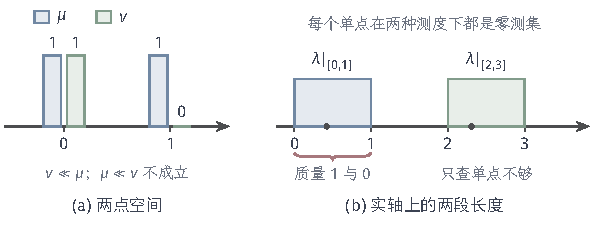
\includegraphics[width=100.669mm]{figures/02-abstract-mathematics/01-metric-and-measure/tikz/c2-absolute-continuity/figure.pdf}
  \caption{绝对连续比较的是零测集。(a)两点空间上$\mu=\delta_0+\delta_1$（蓝）与$\nu=\delta_0$（绿）：$\mu$只把空集看作零测集，所以$\nu\ll\mu$；$\nu$在点$1$的质量为零而$\mu$不为零，所以反向不成立。(b)$\lambda|_{[0,1]}$（蓝）与$\lambda|_{[2,3]}$（绿）在每个单点上都为零，但在$[0,1]$上分别为$1$与$0$，两者互不绝对连续。}
  \label{fig:measure-absolute-continuity}
\end{figure}

\paragraph{小质量控制}
“绝对连续”这个名字来自一个与函数连续性相似的说法：参考测度很小的集合，目标测度也很小。零测集的包含关系是“等于零推出等于零”，下面的定理把它加强为“接近零推出接近零”，但需要目标测度有限。

\begin{theorem}[绝对连续的小质量刻画]
\label{thm:measure-ac-epsilon-delta}
设$\mu,\nu$是$(X,\mathcal A)$上的非负测度，且$\nu$有限。则$\nu\ll\mu$当且仅当：对每个$\varepsilon>0$，存在$\delta>0$，使得对所有$A\in\mathcal A$，
\[
 \mu(A)<\delta\ \Longrightarrow\ \nu(A)<\varepsilon .
\]
\end{theorem}

\begin{proof}
先证充分性。设小质量条件成立，$\mu(A)=0$。对任意$\varepsilon>0$，取相应的$\delta$，则$\mu(A)=0<\delta$，故$\nu(A)<\varepsilon$。$\varepsilon$任意，所以$\nu(A)=0$。

再证必要性，用反证法。设$\nu\ll\mu$而小质量条件不成立，则存在某个$\varepsilon>0$，使得无论$\delta$取多小都有反例。依次取$\delta=2^{-n}$，得到可测集$A_n$满足
\[
 \mu(A_n)<2^{-n},\qquad \nu(A_n)\ge\varepsilon,\qquad n=1,2,\dots .
\]
这些集合的$\mu$质量趋于零，但$\nu$质量不趋于零。为了得到一个$\mu$零测而$\nu$质量为正的集合，考察尾并$B_k=\bigcup_{n\ge k}A_n$。由可数次可加性，
\[
 \mu(B_k)\le\sum_{n\ge k}2^{-n}=2^{1-k},
\]
同时$B_k\supseteq A_k$给出$\nu(B_k)\ge\varepsilon$。

尾并$B_1\supseteq B_2\supseteq\cdots$递减，令$B=\bigcap_kB_k$。对每个$k$有$\mu(B)\le\mu(B_k)\le2^{1-k}$，所以$\mu(B)=0$。另一方面，$\nu$有限，可以对递减集合列使用从上连续性（第~\ref{sec:measure-spaces-def}节），得$\nu(B)=\lim_k\nu(B_k)\ge\varepsilon>0$。这与$\nu\ll\mu$矛盾。
\end{proof}

证明中唯一用到$\nu$有限的地方是从上连续性。这个条件不能去掉。在$X=(0,1]$上取$I_k=(2^{-k},2^{1-k}]$，$k=1,2,\dots$，它们两两不交且并为$(0,1]$。令
\[
 \nu=\sum_{k=1}^\infty 2^k\lambda|_{I_k},\qquad\text{即}\quad \nu(A)=\sum_{k=1}^\infty 2^k\lambda(A\cap I_k),
\]
这是第~\ref{sec:measure-spaces-def}节中测度的可数加权和，仍是测度。若$\lambda(A)=0$，则每项$\lambda(A\cap I_k)=0$，所以$\nu(A)=0$，即$\nu\ll\lambda$。但$\lambda(I_k)=2^{-k}\to0$，而$\nu(I_k)=2^k\cdot2^{-k}=1$对每个$k$成立，小质量条件对$\varepsilon=1$失败。图~\ref{fig:measure-absolute-continuity-blocks}画出了前几块。这里$\nu((0,1])=\sum_k1=+\infty$，$\nu$不是有限测度，与定理并不矛盾。

\begin{figure}[!htbp]
  \centering
  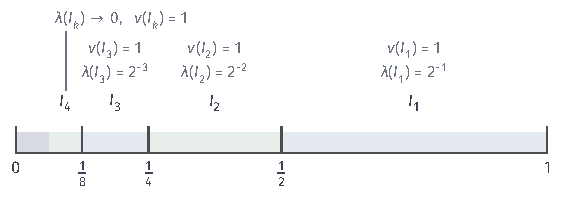
\includegraphics[width=95.324mm]{figures/02-abstract-mathematics/01-metric-and-measure/tikz/c2-absolute-continuity-blocks/figure.pdf}
  \caption{无限测度下小质量控制可能失败。$(0,1]$被分成$I_k=(2^{-k},2^{1-k}]$，它们的长度$\lambda(I_k)=2^{-k}$趋于零，而$\nu=\sum_k2^k\lambda|_{I_k}$给每块的质量都是$1$。$\nu\ll\lambda$成立，但长度小的集合不一定$\nu$质量小。}
  \label{fig:measure-absolute-continuity-blocks}
\end{figure}

\subsection{相互奇异}
\label{sec:measure-mutual-singularity}

绝对连续描述的是“一种测度忽略的地方，另一种也忽略”。与它相对的另一种极端是：两种质量各自待在对方忽略的区域里，互不重叠。

\paragraph{质量集中在不交的可测区域}
若$\nu(X\setminus N)=0$，就说$\nu$\emph{集中}在可测集$N$上：$N$之外没有$\nu$质量。两种测度可以分别集中在一个集合及其补集上。

\begin{definition}[相互奇异]
\label{def:measure-singular}
设$\mu,\nu$是$(X,\mathcal A)$上的非负测度。若存在$N\in\mathcal A$，使
\[
 \mu(N)=0,\qquad \nu(X\setminus N)=0,
\]
就称$\mu$与$\nu$\term{相互奇异}（mutually singular），记作$\mu\perp\nu$。
\end{definition}

定义里$\mu$与$\nu$的地位看似不同，实际是对称的：令$N'=X\setminus N$，则$\nu(N')=0$且$\mu(X\setminus N')=\mu(N)=0$，所以同一关系从$\nu$的角度看就是用补集$N'$作分割。直观地说，$X$被分成两个可测区域，$\nu$的全部质量在$N$中，$\mu$的全部质量在$N'$中。

最直接的例子是长度与点质量。在实轴上取$\mu=\lambda|_{[0,1]}$，$\nu=\tfrac12\delta_{1/2}$，令$N=\{1/2\}$，则$\mu(N)=0$，$\nu(\mathbb R\setminus N)=0$，所以$\mu\perp\nu$，见图~\ref{fig:measure-mutually-singular}(a)。注意点$1/2$恰好位于$[0,1]$的内部：相互奇异不要求两种质量在位置上分开，只要求存在一个可测集合把它们分开。

相互奇异与绝对连续几乎不能同时成立。若$\nu\ll\mu$且$\nu\perp\mu$，取定义中的$N$，则$\mu(N)=0$推出$\nu(N)=0$，再加上$\nu(X\setminus N)=0$，得$\nu(X)=0$，即$\nu$是零测度。这个简单事实将在第~\ref{sec:measure-decomposition}节证明分解唯一时用到。

\paragraph{可测分离不等于距离分离}
在实轴上，“相互奇异”很容易被想象成两团质量隔着一段距离。下面的例子说明这种想象不对。设$(q_n)_{n\ge1}$列举$\mathbb Q$中的全部有理数，令
\[
 \mu=\sum_{n=1}^\infty2^{-n}\delta_{q_n},\qquad
 \nu=\sum_{n=1}^\infty2^{-n}\delta_{q_n+\sqrt2},
\]
两者都是总质量为$\sum_n2^{-n}=1$的有限测度。$\mu$集中在$\mathbb Q$上，$\nu$集中在$\mathbb Q+\sqrt2=\{q+\sqrt2:q\in\mathbb Q\}$上。这两个集合不相交：若$q=q'+\sqrt2$，则$\sqrt2=q-q'$是有理数，矛盾。于是取$N=\mathbb Q+\sqrt2$，有$\mu(N)=0$，$\nu(\mathbb R\setminus N)=0$，$\mu\perp\nu$。

另一方面，$\mathbb Q$与$\mathbb Q+\sqrt2$都在实轴上稠密：每个非空开区间$(a,b)$中既有有理数$q_n$，也有形如$q_m+\sqrt2$的点（取$(a-\sqrt2,b-\sqrt2)$中的有理数$q_m$）。所以$\mu((a,b))\ge2^{-n}>0$且$\nu((a,b))\ge2^{-m}>0$，两种测度在每个非空开区间上都有正质量。图~\ref{fig:measure-mutually-singular}(b)画出了两组点中的前几个，它们彼此交错。可见相互奇异是可测集合层面的分离，与第~\ref{chap:metric-spaces}章的距离结构无关。顺带一提，$\mu$与$\nu$都集中在可数集上，而可数集是Lebesgue零测集，所以它们与$\lambda$也都相互奇异。

\begin{figure}[!htbp]
  \centering
  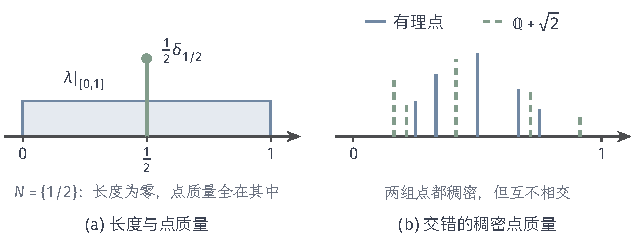
\includegraphics[width=107.668mm]{figures/02-abstract-mathematics/01-metric-and-measure/tikz/c2-mutually-singular/figure.pdf}
  \caption{相互奇异是可测集合上的分离。(a)$\lambda|_{[0,1]}$与$\tfrac12\delta_{1/2}$相互奇异，分离集$N=\{1/2\}$位于区间内部。(b)$\mu=\sum_n2^{-n}\delta_{q_n}$集中在有理点上（蓝色实线），$\nu=\sum_n2^{-n}\delta_{q_n+\sqrt2}$集中在$\mathbb Q+\sqrt2$上（绿色虚线）；图中只画出$[0,1]$内各几个点，线高仅示意权重递减。两组点在每个开区间中都出现，但互不相交，所以$\mu\perp\nu$。}
  \label{fig:measure-mutually-singular}
\end{figure}

\section{测度的差}
\label{sec:measure-signed}

上一节只问两种测度是否忽略相同的集合。若要知道它们在每个集合上差多少，最直接的办法是作差：对两个有限测度$\nu,\mu$，令$\eta(A)=\nu(A)-\mu(A)$。这个赋值可以为正，也可以为负。本节研究这类赋值：它在哪里取正、在哪里取负，能否唯一地写回两个非负测度之差，以及怎样度量它的变化总量。积分尚未定义，本节不讨论对有符号测度的积分。

\subsection{有限有符号测度}
\label{sec:measure-signed-finite}

\paragraph{从测度之差到有符号赋值}
设$\nu,\mu$是$(X,\mathcal A)$上的有限测度，$\eta=\nu-\mu$。对两两不交的可测集$A_1,A_2,\dots$，两个测度各自可数可加，且两个级数都收敛到有限值，所以
\[
 \eta\Bigl(\bigcup_nA_n\Bigr)=\sum_n\nu(A_n)-\sum_n\mu(A_n)=\sum_n\bigl(\nu(A_n)-\mu(A_n)\bigr)=\sum_n\eta(A_n).
\]
可见$\eta$保留了可数可加性，只是不再非负。把这两条性质单独抽出来，就得到下面的定义。

\begin{definition}[有限有符号测度]
\label{def:measure-signed}
可测空间$(X,\mathcal A)$上的\term{有符号测度}（signed measure）$\eta$是映射$\eta:\mathcal A\to\mathbb R$，满足$\eta(\varnothing)=0$，并且对任意两两不交的$A_1,A_2,\dots\in\mathcal A$，级数$\sum_n\eta(A_n)$收敛且
\[
 \eta\Bigl(\bigcup_{n=1}^\infty A_n\Bigr)=\sum_{n=1}^\infty\eta(A_n).
\]
本书只讨论取有限实值的情形，称为有限有符号测度。
\end{definition}

不交集合的并与排列次序无关，所以上式右端的级数无论怎样重排都收敛到同一个值；按实数级数的重排定理，这意味着它绝对收敛。本章后面只用到一个更弱的推论：级数收敛，其通项必须趋于零。

有符号测度是给\emph{集合}赋予实数的规则，不要与在某些\emph{点}上取负值的实值函数混淆。$\eta(A)<0$表示集合$A$上的“负质量”多于“正质量”，这个数由整个集合决定，而不是由某一点的取值决定。要求取有限值，是为了避免出现$+\infty-\infty$：两个无限测度作差时，$\nu(A)-\mu(A)$可能根本没有定义。

\begin{example}[正负抵消]
\label{ex:measure-signed-weights}
取$X=\{1,2,3,4\}$及全部子集，规定单点值
\[
 \eta(\{1\})=2,\quad \eta(\{2\})=-1,\quad \eta(\{3\})=1,\quad \eta(\{4\})=-2,
\]
并令$\eta(A)=\sum_{i\in A}\eta(\{i\})$。有限集上的这种加和自动满足可加性，所以$\eta$是有符号测度；它也可以写成$\eta=\nu-\mu$，其中$\nu=2\delta_1+\delta_3$，$\mu=\delta_2+2\delta_4$。

计算几个值：$\eta(X)=2-1+1-2=0$，$\eta(\{1,2\})=1$，$\eta(\{1,3\})=3$，$\eta(\{2,4\})=-3$。全空间上的值为零，但这只是正负抵消的结果；在$\{1,3\}$与$\{2,4\}$上，$\eta$的绝对值都达到$3$。所以$\eta(X)$很小甚至为零，不能说明$\eta$在各处都小。图~\ref{fig:measure-signed-weights}把四个权重画成向上、向下的柱。
\end{example}

\begin{figure}[!htbp]
  \centering
  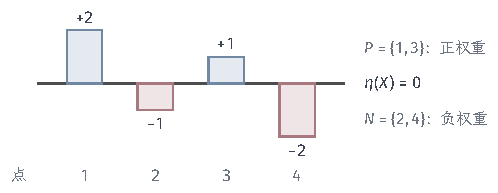
\includegraphics[width=84.36mm]{figures/02-abstract-mathematics/01-metric-and-measure/tikz/c2-signed-weights/figure.pdf}
  \caption{四点集合上的有符号测度。蓝色柱向上表示正权重，红色柱向下表示负权重。正负相互抵消使$\eta(X)=0$，但$\eta$在$P=\{1,3\}$上为$3$，在$N=\{2,4\}$上为$-3$。}
  \label{fig:measure-signed-weights}
\end{figure}

例中的$\eta$还有另一种写法：$\eta=(\nu+\delta_1)-(\mu+\delta_1)$。同一个有符号测度可以有许多种“正测度减正测度”的表示。下一小节要找的是其中一种由$\eta$本身确定、没有多余抵消的表示。

\subsection{Hahn分解与Jordan分解}
\label{sec:measure-hahn-jordan}

例~\ref{ex:measure-signed-weights}中，只要把$X$分成$\{1,3\}$与$\{2,4\}$，$\eta$在前一部分的每个子集上都非负，在后一部分的每个子集上都非正。一般的有符号测度是否也能这样一刀切成正、负两个区域？这正是Hahn分解回答的问题。

\paragraph{正集与负集}
只看$\eta(P)\ge0$并不够：在例~\ref{ex:measure-signed-weights}中$\eta(\{1,2\})=1\ge0$，但它的子集$\{2\}$取值为$-1$。我们需要的是对所有子集都保持符号的集合。

\begin{definition}[正集与负集]
\label{def:measure-positive-set}
设$\eta$是$(X,\mathcal A)$上的有限有符号测度。若$P\in\mathcal A$的每个可测子集$E$都满足$\eta(E)\ge0$，称$P$为$\eta$的\term{正集}（positive set）；若$N\in\mathcal A$的每个可测子集$E$都满足$\eta(E)\le0$，称$N$为$\eta$的\term{负集}（negative set）。
\end{definition}

正集的可测子集仍是正集，可数个正集的并也是正集：若$P_1,P_2,\dots$是正集，$E\subseteq\bigcup_nP_n$可测，令$E_1=E\cap P_1$，$E_n=E\cap P_n\setminus(P_1\cup\dots\cup P_{n-1})$，则$E_n$是$P_n$的可测子集且两两不交，$\eta(E)=\sum_n\eta(E_n)\ge0$。负集同理。

\paragraph{两条准备性质}
构造正负区域之前，需要两条只依赖可数可加性的性质。第一条说明有限有符号测度的取值不会无限地向下（或向上）延伸，这样“使$\eta$最小的集合”才有可能存在；第二条把测度的单调集合列连续性搬到有符号情形。

\begin{lemma}[有限有符号测度有界]
\label{lem:measure-signed-bounded}
有限有符号测度$\eta$有界：存在$M<\infty$，使$|\eta(A)|\le M$对一切$A\in\mathcal A$成立。
\end{lemma}

\begin{proof}
称可测集$A$是\emph{无界的}，如果$\sup\{|\eta(E)|:E\subseteq A,\ E\in\mathcal A\}=\infty$。设结论不成立，即$X$是无界的。我们将构造两两不交的可测集$B_1,B_2,\dots$，使每个$|\eta(B_n)|\ge1$。

设$A$是无界集。取可测子集$E\subseteq A$使$|\eta(E)|\ge|\eta(A)|+1$，则
\[
 |\eta(A\setminus E)|=|\eta(A)-\eta(E)|\ge|\eta(E)|-|\eta(A)|\ge1 .
\]
于是$E$与$A\setminus E$的取值绝对值都至少为$1$。它们中至少有一个是无界的：否则$A$的任一可测子集$F$满足$|\eta(F)|\le|\eta(F\cap E)|+|\eta(F\setminus E)|$，右边两项都有界，$A$就不是无界的。把无界的那一块记为$A'$，另一块记为$B$，则$B\subseteq A\setminus A'$且$|\eta(B)|\ge1$。

从$A_0=X$出发反复执行这一步，得到无界集$A_0\supseteq A_1\supseteq\cdots$及$B_n\subseteq A_{n-1}\setminus A_n$。由于$B_n\subseteq A_{n-1}\setminus A_n$，而$B_m\subseteq A_{m-1}\subseteq A_n$（$m>n$），这些$B_n$两两不交。按定义~\ref{def:measure-signed}，$\sum_n\eta(B_n)$收敛到$\eta(\bigcup_nB_n)$，通项必须趋于零；但$|\eta(B_n)|\ge1$，矛盾。
\end{proof}

\begin{lemma}[有符号测度的单调连续性]
\label{lem:measure-signed-continuity}
设$\eta$是有限有符号测度。若$A_1\subseteq A_2\subseteq\cdots$，则$\eta(\bigcup_nA_n)=\lim_n\eta(A_n)$；若$A_1\supseteq A_2\supseteq\cdots$，则$\eta(\bigcap_nA_n)=\lim_n\eta(A_n)$。
\end{lemma}

\begin{proof}
对递增集合列，令$D_1=A_1$，$D_n=A_n\setminus A_{n-1}$，它们两两不交，$\bigcup_nA_n=\bigcup_nD_n$，且$A_n=D_1\cup\dots\cup D_n$。由可数可加性，$\eta(\bigcup_nA_n)=\sum_n\eta(D_n)$，部分和恰为$\eta(A_n)$，所以等式成立。对递减集合列，$A_1\setminus A_n$递增，并为$A_1\setminus\bigcap_nA_n$；由已证部分及有限可加性$\eta(A_1\setminus B)=\eta(A_1)-\eta(B)$（$B\subseteq A_1$，各项有限），得$\eta(A_1)-\eta(\bigcap_nA_n)=\lim_n(\eta(A_1)-\eta(A_n))$。
\end{proof}

与非负测度不同，这里递减情形不需要另加有限性假设，因为$\eta$本身只取有限值。

\paragraph{Hahn分解}
思路是寻找使$\eta$取最小值的可测集$D$。若某个$D$达到最小值，那么从$D$中拿走一个正值子集，或向$D$中添入一个负值的外部集合，都会让取值更小，这不可能；于是$D$自然是负集，补集是正集。难点在于证明最小值确实能被某个集合达到。

\begin{theorem}[Hahn分解]
\label{thm:measure-hahn}
设$\eta$是$(X,\mathcal A)$上的有限有符号测度。则存在$P\in\mathcal A$，使$P$是$\eta$的正集，$N=X\setminus P$是$\eta$的负集。这样的一对$(P,N)$称为$\eta$的\term{Hahn分解}（Hahn decomposition）。若$(P',N')$是另一组Hahn分解，则$P\cap N'$与$P'\cap N$的每个可测子集上$\eta$都取零。
\end{theorem}

\begin{proof}
令$m=\inf_{A\in\mathcal A}\eta(A)$。由引理~\ref{lem:measure-signed-bounded}，$m$是有限实数；又$\eta(\varnothing)=0$，故$m\le0$。对每个$n$取可测集$A_n$使$\eta(A_n)<m+2^{-n}$。

第一步说明两个“近乎最小”的集合取交后仍近乎最小。对可测集$A,B$，有限可加性给出$\eta(A\cup B)+\eta(A\cap B)=\eta(A)+\eta(B)$；又$\eta(A\cup B)\ge m$，所以
\[
 \eta(A\cap B)\le\eta(A)+\eta(B)-m .
\]
固定$n$，对$k\ge n$令$C_{n,k}=A_n\cap A_{n+1}\cap\dots\cap A_k$。对$k$归纳，并利用上式，
\[
 \eta(C_{n,k+1})\le\eta(C_{n,k})+\eta(A_{k+1})-m<m+\sum_{j=n}^{k+1}2^{-j}.
\]
所以$\eta(C_{n,k})<m+2^{1-n}$对所有$k\ge n$成立。

第二步取极限。$C_{n,k}$关于$k$递减，令$C_n=\bigcap_{k\ge n}A_k$；由引理~\ref{lem:measure-signed-continuity}，$\eta(C_n)=\lim_k\eta(C_{n,k})\le m+2^{1-n}$。$C_n$关于$n$递增，令$D=\bigcup_nC_n$；再由引理~\ref{lem:measure-signed-continuity}，$\eta(D)=\lim_n\eta(C_n)\le m$。另一方面$\eta(D)\ge m$，所以$\eta(D)=m$，最小值被$D$达到。

第三步验证符号。若可测集$E\subseteq D$满足$\eta(E)>0$，则$\eta(D\setminus E)=m-\eta(E)<m$，与$m$是下确界矛盾，所以$D$是负集。若可测集$E\subseteq X\setminus D$满足$\eta(E)<0$，则$\eta(D\cup E)=m+\eta(E)<m$，同样矛盾，所以$X\setminus D$是正集。取$N=D$，$P=X\setminus D$即可。

最后看两组分解的差别。$P\cap N'$既是正集$P$的子集，又是负集$N'$的子集，它的每个可测子集$E$同时满足$\eta(E)\ge0$与$\eta(E)\le0$，即$\eta(E)=0$。$P'\cap N$同理。
\end{proof}

整个证明只用了集合运算、有限可加性与单调连续性。Hahn分解一般不唯一：$\eta$在其上“完全为零”的区域可以划给任意一侧。例如在实轴上令$\eta=\lambda|_{[0,1]}-\lambda|_{[2,3]}$，$P_1=(-\infty,3/2)$与$P_2=(-\infty,2)$都给出Hahn分解，两者相差的$[3/2,2)$上$\eta$的每个子集都取零，见图~\ref{fig:measure-hahn-decomposition}。正区域还可以只差一个Lebesgue零测集，例如把点$1/2$从$P_1$移到负区域一侧。

\begin{figure}[!htbp]
  \centering
  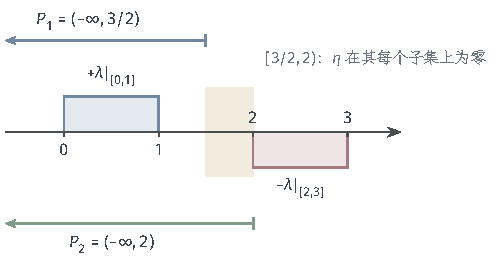
\includegraphics[width=84.06mm]{figures/02-abstract-mathematics/01-metric-and-measure/tikz/c2-hahn-decomposition/figure.pdf}
  \caption{Hahn分解的区域选择不唯一。$\eta=\lambda|_{[0,1]}-\lambda|_{[2,3]}$，蓝块在$[0,1]$上表示正的长度，红块在$[2,3]$上表示负的长度，块高表示长度测度前的系数$\pm1$。正区域可以取$P_1=(-\infty,3/2)$，也可以取$P_2=(-\infty,2)$；二者之差$[3/2,2)$（黄色）的每个可测子集上$\eta$都为零，所以放在哪一侧都不改变符号要求。}
  \label{fig:measure-hahn-decomposition}
\end{figure}

\paragraph{Jordan分解}
区域可以不同，但限制在区域上的质量却是唯一的。把$\eta$分别限制到正区域与负区域，就得到两个非负测度。

\begin{theorem}[Jordan分解]
\label{thm:measure-jordan}
设$\eta$是有限有符号测度，$(P,N)$是它的一组Hahn分解。令
\[
 \eta^+(A)=\eta(A\cap P),\qquad \eta^-(A)=-\eta(A\cap N),\qquad A\in\mathcal A .
\]
则$\eta^+,\eta^-$是有限非负测度，$\eta=\eta^+-\eta^-$，且$\eta^+\perp\eta^-$；它们不依赖于Hahn分解的选取。反过来，若$\eta=\alpha-\beta$，其中$\alpha,\beta$是相互奇异的有限非负测度，则$\alpha=\eta^+$，$\beta=\eta^-$。这个唯一的表示称为$\eta$的\term{Jordan分解}（Jordan decomposition），$\eta^+$、$\eta^-$分别称为$\eta$的正部分与负部分。
\end{theorem}

\begin{proof}
$A\cap P$是正集的子集，所以$\eta^+(A)\ge0$；同理$\eta^-(A)\ge0$。两者的可数可加性直接来自$\eta$：若$A_n$两两不交，则$A_n\cap P$也两两不交。由$A=(A\cap P)\cup(A\cap N)$得$\eta(A)=\eta^+(A)-\eta^-(A)$。又$\eta^+(N)=\eta(\varnothing)=0$，$\eta^-(X\setminus N)=\eta^-(P)=0$，所以$\eta^+\perp\eta^-$。

再看与Hahn分解无关。设$(P',N')$是另一组分解。由定理~\ref{thm:measure-hahn}，$A\cap P\cap N'$与$A\cap P'\cap N$上$\eta$取零，因此
\[
 \eta(A\cap P)=\eta(A\cap P\cap P')+\eta(A\cap P\cap N')=\eta(A\cap P\cap P')=\eta(A\cap P'),
\]
最后一步对$P'$作同样的拆分。$\eta^-$同理。

最后证唯一性。设$\eta=\alpha-\beta$且$\alpha\perp\beta$，按定义~\ref{def:measure-singular}取可测集$S$使$\beta(S)=0$，$\alpha(X\setminus S)=0$。对$S$的可测子集$E$，$\eta(E)=\alpha(E)-\beta(E)=\alpha(E)\ge0$；对$X\setminus S$的可测子集$E$，$\eta(E)=-\beta(E)\le0$。所以$(S,X\setminus S)$本身是一组Hahn分解。由已证的无关性，
\[
 \eta^+(A)=\eta(A\cap S)=\alpha(A\cap S)=\alpha(A),
\]
其中最后一步用了$\alpha(A\setminus S)=0$。同理$\beta=\eta^-$。
\end{proof}

Jordan分解的唯一性依赖“相互奇异”这一条件。任意两个有限测度之差都是有符号测度，但一般不是Jordan分解。仍取$\eta=\lambda|_{[0,1]}-\lambda|_{[2,3]}$，它的Jordan部分是$\eta^+=\lambda|_{[0,1]}$、$\eta^-=\lambda|_{[2,3]}$。另一方面，令
\[
 \alpha=\lambda|_{[0,3]},\qquad \beta=\lambda|_{[1,2]}+2\lambda|_{[2,3]},
\]
逐段检查：在$[0,1]$上$\alpha-\beta$的系数为$1-0=1$，在$[1,2]$上为$1-1=0$，在$[2,3]$上为$1-2=-1$，所以同样有$\alpha-\beta=\eta$。但$\alpha$与$\beta$在$[1,3]$上重叠，并不相互奇异，且$\alpha(\mathbb R)=\beta(\mathbb R)=3$，而$\eta^\pm(\mathbb R)=1$，见图~\ref{fig:measure-jordan-decomposition}。

这种多余的重叠总是只增不减。对任意表示$\eta=\alpha-\beta$（$\alpha,\beta$为有限非负测度）及任意$A\in\mathcal A$，
\[
 \eta^+(A)=\eta(A\cap P)=\alpha(A\cap P)-\beta(A\cap P)\le\alpha(A\cap P)\le\alpha(A),
\]
同理$\eta^-(A)\le\beta(A)$。所以Jordan分解是所有“正测度减正测度”表示中最小的一个。取$\alpha=\eta^+$时等号成立，于是还得到正部分的一个不依赖于Hahn分解的读法：
\[
 \eta^+(A)=\sup\{\eta(E):E\subseteq A,\ E\in\mathcal A\},
\]
因为每个$\eta(E)=\eta^+(E)-\eta^-(E)\le\eta^+(E)\le\eta^+(A)$，而$E=A\cap P$达到这个上界。

\begin{figure}[!htbp]
  \centering
  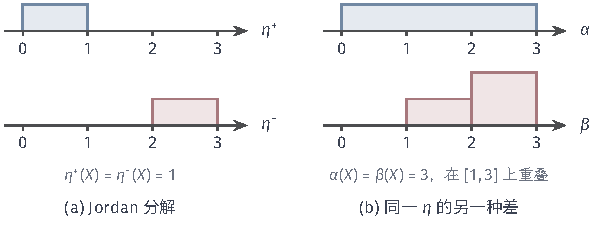
\includegraphics[width=101.745mm]{figures/02-abstract-mathematics/01-metric-and-measure/tikz/c2-jordan-decomposition/figure.pdf}
  \caption{同一个有符号测度$\eta=\lambda|_{[0,1]}-\lambda|_{[2,3]}$的两种差表示，块高为长度测度前的系数。(a)Jordan分解：$\eta^+$与$\eta^-$分别集中在$[0,1]$与$[2,3]$上，相互奇异，总质量各为$1$。(b)$\alpha=\lambda|_{[0,3]}$与$\beta=\lambda|_{[1,2]}+2\lambda|_{[2,3]}$之差也等于$\eta$，但两者在$[1,3]$上重叠，总质量各为$3$。}
  \label{fig:measure-jordan-decomposition}
\end{figure}

\subsection{总变差测度}
\label{sec:measure-total-variation}

$|\eta(A)|$衡量的是集合$A$上正负相抵后的净值；例~\ref{ex:measure-signed-weights}说明它可能掩盖很大的局部变化。若要累计正负两方面的全部质量，就应当把正部分与负部分相加，而不是相减。

\paragraph{定义与分割刻画}

\begin{definition}[总变差测度]
\label{def:measure-total-variation}
设$\eta$是有限有符号测度，$\eta=\eta^+-\eta^-$是它的Jordan分解。称
\[
 |\eta|=\eta^++\eta^-
\]
为$\eta$的\term{总变差测度}（total variation measure），称$|\eta|(X)$为$\eta$的总变差。
\end{definition}

$|\eta|$是两个有限非负测度之和，所以仍是有限非负测度。它也可以不借助Jordan分解，而直接从$\eta$的取值读出：把$A$切成有限块，对每块的净值取绝对值再相加，切得越合适，抵消越少。

\begin{theorem}[总变差的分割刻画]
\label{thm:measure-total-variation-partition}
对每个$A\in\mathcal A$，
\[
 \begin{aligned}
  |\eta|(A)=\sup\Bigl\{\sum_{i=1}^k|\eta(A_i)|:\ &k\ge1,\ A_1,\dots,A_k\in\mathcal A\text{两两不交},\\
  &\bigcup_{i=1}^kA_i=A\Bigr\}.
 \end{aligned}
\]
\end{theorem}

\begin{proof}
对$A$的任一有限可测分割，
\[
 \sum_i|\eta(A_i)|=\sum_i|\eta^+(A_i)-\eta^-(A_i)|\le\sum_i\bigl(\eta^+(A_i)+\eta^-(A_i)\bigr)=|\eta|(A),
\]
最后一步用了$\eta^\pm$的有限可加性。所以上确界不超过$|\eta|(A)$。取Hahn分解$(P,N)$及分割$A_1=A\cap P$、$A_2=A\cap N$，则$|\eta(A_1)|+|\eta(A_2)|=\eta^+(A)+\eta^-(A)=|\eta|(A)$，上确界被达到。
\end{proof}

回到例~\ref{ex:measure-signed-weights}。不分割时$|\eta(X)|=0$；分成$\{1,2\}$与$\{3,4\}$时得$|1|+|-1|=2$；分成$\{1,3\}$与$\{2,4\}$时得$|3|+|-3|=6$。再细分也不会超过$6$，因为四个单点上的绝对值之和为$2+1+1+2=6$。所以$|\eta|(X)=6$，正好由正负区域的分割取得，见图~\ref{fig:measure-total-variation-partition}。

\begin{figure}[!htbp]
  \centering
  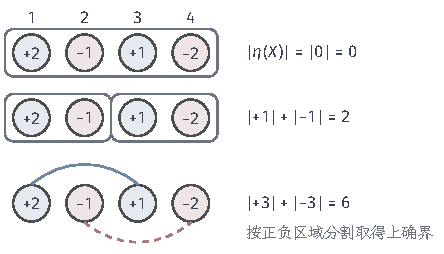
\includegraphics[width=75.128mm]{figures/02-abstract-mathematics/01-metric-and-measure/tikz/c2-total-variation-partition/figure.pdf}
  \caption{用分割读取总变差。四个点的权重为$+2,-1,+1,-2$。第一行不分割，净值为$0$；第二行把相邻的正负点合在一起，仍有抵消，绝对值之和为$2$；第三行按符号分组（蓝色实弧连接正点，红色虚弧连接负点），没有抵消，绝对值之和为$6=|\eta|(X)$。}
  \label{fig:measure-total-variation-partition}
\end{figure}

\paragraph{净值与总量}
由分割刻画取平凡分割$\{A\}$，立即得到
\[
 |\eta(A)|\le|\eta|(A),\qquad A\in\mathcal A .
\]
左边允许抵消，右边累计正负变化的总量。特别地，$|\eta|(A)=0$当且仅当$\eta$在$A$的每个可测子集上都取零：必要性来自上面的不等式用于子集，充分性来自分割刻画中每一项都为零。因此$|\eta|$的零测集正是$\eta$“完全看不见”的集合；后面讨论有符号测度时，“几乎处处”都相对于$|\eta|$来理解。

对两个概率测度$P,Q$，差$\eta=P-Q$满足$\eta(X)=0$，于是$\eta^+(X)=\eta^-(X)=\tfrac12|\eta|(X)$；再由正部分的上确界读法，
\[
 \tfrac12|P-Q|(X)=\eta^+(X)=\sup_{A\in\mathcal A}\bigl(P(A)-Q(A)\bigr).
\]
这个量在后续比较概率分布时称为全变差距离，它与其他分布距离的关系留到讨论概率分布的部分。第~\ref{chap:integration}章将用$|\eta|$为有符号测度的积分规定绝对可积条件，第~\ref{chap:densities-change-of-measure}章则研究$\eta$何时能由一个可积函数表示。

\section{测度的分解}
\label{sec:measure-decomposition}

第~\ref{sec:measure-relations}节的两种关系是两个极端：$\nu\ll\mu$时，$\nu$完全不在$\mu$的零测集上放质量；$\nu\perp\mu$时，$\nu$的全部质量都放在某个$\mu$零测集上。一般的测度介于两者之间，例如长度加上一个点质量。本节先证明：相对于给定的参考测度，任何$\sigma$有限测度都能唯一地拆成这两种极端之和；再在实轴上以Lebesgue测度为参考，把奇异部分进一步拆成点质量与“没有点质量的奇异质量”，并用Cantor集具体构造后者。整节只使用测度，不要求绝对连续部分能写成密度。

\subsection{Lebesgue分解}
\label{sec:measure-lebesgue-decomposition}

\paragraph{分解的陈述}
给定参考测度$\mu$与目标测度$\nu$，我们希望把$\nu$的质量分成两份：一份完全落在某个$\mu$零测集上，另一份在$\mu$零测集上没有任何质量。前者是$\mu$“看不见”的质量，后者是$\mu$能够“看见”的质量。

\begin{theorem}[Lebesgue分解]
\label{thm:measure-lebesgue-decomposition}
设$\mu$是可测空间$(X,\mathcal A)$上的非负测度，$\nu$是同一空间上的$\sigma$有限非负测度。则存在唯一的一对非负测度$\nu_{\mathrm{ac}},\nu_{\mathrm{s}}$，使
\[
 \nu=\nu_{\mathrm{ac}}+\nu_{\mathrm{s}},\qquad \nu_{\mathrm{ac}}\ll\mu,\qquad \nu_{\mathrm{s}}\perp\mu .
\]
这称为$\nu$相对于$\mu$的\term{Lebesgue分解}（Lebesgue decomposition），$\nu_{\mathrm{ac}}$与$\nu_{\mathrm{s}}$分别称为绝对连续部分与奇异部分。更具体地，存在$N\in\mathcal A$使$\mu(N)=0$，并且$\nu_{\mathrm{s}}(A)=\nu(A\cap N)$，$\nu_{\mathrm{ac}}(A)=\nu(A\setminus N)$。
\end{theorem}

分解总是相对于参考测度的。在实轴上取$\nu=\lambda|_{[0,1]}+\delta_2$。以$\lambda$为参考时，$N=\{2\}$是$\lambda$零测集且承载点质量，于是$\nu_{\mathrm{s}}=\delta_2$，$\nu_{\mathrm{ac}}=\lambda|_{[0,1]}$。以$\delta_2$为参考时，$\delta_2$的零测集是不含点$2$的集合，取$N=\mathbb R\setminus\{2\}$，于是角色互换：$\nu_{\mathrm{s}}=\lambda|_{[0,1]}$，$\nu_{\mathrm{ac}}=\delta_2$。同一个$\nu$换一个参考，同一份质量就可能从一个部分换到另一个部分，见图~\ref{fig:measure-lebesgue-decomposition}。

\begin{figure}[!htbp]
  \centering
  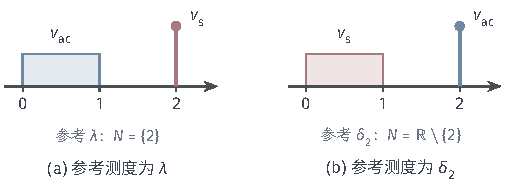
\includegraphics[width=85.672mm]{figures/02-abstract-mathematics/01-metric-and-measure/tikz/c2-lebesgue-decomposition/figure.pdf}
  \caption{Lebesgue分解依赖参考测度。$\nu=\lambda|_{[0,1]}+\delta_2$，蓝色为绝对连续部分，红色为奇异部分。(a)以$\lambda$为参考，点$2$是$\lambda$零测集，点质量是奇异部分；(b)以$\delta_2$为参考，$\mathbb R\setminus\{2\}$是$\delta_2$零测集，区间上的长度变成奇异部分。}
  \label{fig:measure-lebesgue-decomposition}
\end{figure}

\paragraph{有限情形：选取承载最多质量的零测集}
定理中的集合$N$应当尽可能多地装下$\nu$的质量，同时保持$\mu(N)=0$。若某个$\mu$零测集在$N$之外还有正的$\nu$质量，就把它并进$N$。这个“装到不能再装”的想法可以用上确界实现。我们先在$\nu$有限时证明存在性。

\begin{proof}[定理~\ref{thm:measure-lebesgue-decomposition}在$\nu$有限时的存在性]
令
\[
 M=\sup\{\nu(A):A\in\mathcal A,\ \mu(A)=0\}.
\]
空集在集合族中，所以$M\ge0$；又$M\le\nu(X)<\infty$。对每个$k$取$\mu$零测集$N_k$使$\nu(N_k)>M-1/k$，并令$N=\bigcup_kN_k$。由可数次可加性，$\mu(N)\le\sum_k\mu(N_k)=0$，所以$N$本身也在集合族中，$\nu(N)\le M$；另一方面$\nu(N)\ge\nu(N_k)>M-1/k$对每个$k$成立，故$\nu(N)=M$。上确界被$N$达到。

令$\nu_{\mathrm{s}}(A)=\nu(A\cap N)$，$\nu_{\mathrm{ac}}(A)=\nu(A\setminus N)$。两者都是$\nu$限制到可测子集所得的测度，且$\nu=\nu_{\mathrm{ac}}+\nu_{\mathrm{s}}$。由$\mu(N)=0$与$\nu_{\mathrm{s}}(X\setminus N)=0$得$\nu_{\mathrm{s}}\perp\mu$。

剩下证明$\nu_{\mathrm{ac}}\ll\mu$。设$\mu(A)=0$，则$N\cup(A\setminus N)$仍是$\mu$零测集，其$\nu$质量不超过$M$。这两部分不交，所以
\[
 M+\nu(A\setminus N)=\nu(N)+\nu(A\setminus N)\le M .
\]
$M$有限，可以从两边消去，得$\nu_{\mathrm{ac}}(A)=\nu(A\setminus N)=0$。
\end{proof}

最后一步的“消去”正是需要$\nu$有限的地方：若$M=+\infty$，不等式$M+t\le M$不能推出$t=0$。

\paragraph{$\sigma$有限情形与唯一性}
$\sigma$有限测度可以切成可数个有限片，在每片上重复上面的构造，再把各片的零测集合并。

\begin{proof}[定理~\ref{thm:measure-lebesgue-decomposition}在一般情形下的存在性与唯一性]
\emph{存在性。}由$\sigma$有限性，取两两不交的$X_1,X_2,\dots\in\mathcal A$使$\bigcup_jX_j=X$且$\nu(X_j)<\infty$。对每个$j$，有限测度$\nu_j(A)=\nu(A\cap X_j)$满足已证情形，得到$\mu$零测集$N_j'$；用$N_j=N_j'\cap X_j$代替它，仍有$\mu(N_j)=0$，且$\nu_j(A\setminus N_j)=\nu_j(A\setminus N_j')$对所有$A$成立，因为$\nu_j$在$X_j$之外没有质量。令$N=\bigcup_jN_j$，则$\mu(N)=0$。定义$\nu_{\mathrm{s}}(A)=\nu(A\cap N)$，$\nu_{\mathrm{ac}}(A)=\nu(A\setminus N)$，同前有$\nu_{\mathrm{s}}\perp\mu$。若$\mu(A)=0$，由$N\cap X_j=N_j$，
\[
 \nu_{\mathrm{ac}}(A)=\sum_j\nu\bigl((A\setminus N)\cap X_j\bigr)=\sum_j\nu_j(A\setminus N_j)=0,
\]
最后一步是各片上已证的绝对连续性。

\emph{唯一性。}设$\nu=\alpha+\beta=\alpha'+\beta'$，其中$\alpha,\alpha'\ll\mu$，$\beta,\beta'\perp\mu$。取$\mu$零测集$S,S'$使$\beta(X\setminus S)=0$，$\beta'(X\setminus S')=0$，令$T=S\cup S'$，则$\mu(T)=0$，且$\beta,\beta'$在$X\setminus T$上都没有质量。对任意$A\in\mathcal A$，$\mu(A\cap T)=0$推出$\alpha(A\cap T)=\alpha'(A\cap T)=0$，因此
\[
 \beta(A\cap T)=\nu(A\cap T)=\beta'(A\cap T);
\]
又$\beta(A\setminus T)=\beta'(A\setminus T)=0$，因此$\alpha(A\setminus T)=\nu(A\setminus T)=\alpha'(A\setminus T)$。把$A\cap T$与$A\setminus T$上的值相加，得$\alpha=\alpha'$，$\beta=\beta'$。
\end{proof}

唯一性的论证只在两个集合上分别读取$\nu$，没有做减法。整个证明用到的只是可数次可加性、上确界与限制测度，没有用到积分、Hahn分解或任何密度。

存在性中的$\sigma$有限条件不能随意去掉。在$[0,1]$的Borel可测空间上取$\mu=\lambda$，$\nu$为计数测度，它不是$\sigma$有限的（可数个有限测度集都是有限集，并起来只是可数集）。若$\nu=\nu_{\mathrm{ac}}+\nu_{\mathrm{s}}$满足定理的要求，取$N$使$\lambda(N)=0$、$\nu_{\mathrm{s}}([0,1]\setminus N)=0$。由于$\lambda(N)=0$，$N\ne[0,1]$，取$x\notin N$，则$\nu_{\mathrm{s}}(\{x\})=0$，而$\lambda(\{x\})=0$又给出$\nu_{\mathrm{ac}}(\{x\})=0$，于是$\nu(\{x\})=0$，与计数测度给单点质量$1$矛盾。

第~\ref{chap:densities-change-of-measure}章将回答下一个问题：绝对连续部分$\nu_{\mathrm{ac}}$在什么条件下能写成参考测度$\mu$的加权形式。那是在积分建立之后，对已经分出的绝对连续质量寻找函数表示；本节的分解并不依赖它。

\subsection{实轴上的三元分解}
\label{sec:measure-three-part}

在实轴上以Lebesgue测度为参考时，奇异部分还可以再分。单点都是$\lambda$零测集，所以点质量一定属于奇异部分；问题是奇异部分是否只有点质量。下面先把点质量完整地提出来，再说明余下的奇异部分可以不为零。

\paragraph{点质量至多可数}
设$\rho$是$\mathcal B(\mathbb R)$上的有限测度。若$\rho(\{x\})>0$，称$x$是$\rho$的一个原子，即带正质量的单点。

\begin{lemma}[正质量单点至多可数]
\label{lem:measure-atoms-countable}
有限Borel测度$\rho$的原子集$A=\{x\in\mathbb R:\rho(\{x\})>0\}$至多可数。
\end{lemma}

\begin{proof}
按质量的正下界分组：令$A_k=\{x:\rho(\{x\})>1/k\}$，则$A=\bigcup_kA_k$。若$x_1,\dots,x_m$是$A_k$中互不相同的点，有限可加性与单调性给出$m/k<\sum_{i=1}^m\rho(\{x_i\})\le\rho(\mathbb R)$，所以$A_k$至多有$k\rho(\mathbb R)$个点。可数个有限集之并至多可数。
\end{proof}

于是可以定义$\rho_{\mathrm d}(B)=\rho(B\cap A)$。由于$A$至多可数，可数可加性给出
\[
 \rho_{\mathrm d}(B)=\sum_{x\in A\cap B}\rho(\{x\}),
\]
它是全部点质量之和，称为$\rho$的离散部分。余下的$\rho_{\mathrm c}(B)=\rho(B\setminus A)$没有原子：$x\in A$时$\rho_{\mathrm c}(\{x\})=0$，$x\notin A$时$\rho_{\mathrm c}(\{x\})=\rho(\{x\})=0$。

\begin{theorem}[实轴上有限测度的三元分解]
\label{thm:measure-three-part}
设$\rho$是$\mathcal B(\mathbb R)$上的有限测度。则$\rho$可以唯一地写成
\[
 \rho=\rho_{\mathrm d}+\rho_{\mathrm{ac}}+\rho_{\mathrm{sc}},
\]
其中$\rho_{\mathrm d}$集中在一个至多可数集上，$\rho_{\mathrm{ac}}\ll\lambda$，$\rho_{\mathrm{sc}}\perp\lambda$且$\rho_{\mathrm{sc}}$没有原子。没有原子且与$\lambda$相互奇异的测度称为\term{奇异连续测度}（singular continuous measure）。
\end{theorem}

\begin{proof}
存在性：$\rho_{\mathrm d}$与$\rho_{\mathrm c}$如上定义。对有限测度$\rho_{\mathrm c}$关于$\lambda$作Lebesgue分解，得$\rho_{\mathrm c}=\rho_{\mathrm{ac}}+\rho_{\mathrm{sc}}$。$\rho_{\mathrm{sc}}(\{x\})\le\rho_{\mathrm c}(\{x\})=0$，所以$\rho_{\mathrm{sc}}$没有原子。

唯一性：设$\rho=d+a+s$也满足条件，$d$集中在至多可数集$D$上。$a\ll\lambda$与$\lambda(\{x\})=0$给出$a(\{x\})=0$，而$s$没有原子，所以$\rho(\{x\})=d(\{x\})$对每个$x$成立。于是
\[
 d(B)=\sum_{x\in B\cap D}d(\{x\})=\sum_{x\in B\cap D}\rho(\{x\})=\sum_{x\in B\cap A}\rho(\{x\})=\rho_{\mathrm d}(B),
\]
第一个等号用了$d$集中在可数集$D$上及可数可加性。第三个等号成立，是因为$D$中质量为零的点不贡献，而$A\subseteq D$：若$\rho(\{x\})>0$，则$d(\{x\})=\rho(\{x\})>0$，而$d$在$D$之外没有质量，故$x\in D$。由此$a+s=\rho-d=\rho_{\mathrm c}$（各项有限，减法有意义），再由定理~\ref{thm:measure-lebesgue-decomposition}的唯一性得$a=\rho_{\mathrm{ac}}$，$s=\rho_{\mathrm{sc}}$。
\end{proof}

离散部分集中在可数集$A$上，而$\lambda(A)=0$，所以$\rho_{\mathrm d}\perp\lambda$；$\rho$相对于$\lambda$的Lebesgue奇异部分就是$\rho_{\mathrm d}+\rho_{\mathrm{sc}}$。三项是\emph{同一个测度的三个成分}，一个测度可以同时含有三者，也可以缺少其中任意几项；它们不是把测度分成三个互斥类别。

三项中的离散部分可以从累计函数读出。记$G(x)=\rho((-\infty,x])$。集合$(-\infty,x-1/m]$递增到$(-\infty,x)$，由测度从下连续性，$G(x-)=\rho((-\infty,x))$，所以
\[
 G(x)-G(x-)=\rho(\{x\}),
\]
这与第~\ref{sec:measure-construction}节中Lebesgue–Stieltjes测度的单点质量公式一致。因此$G$在$x$处跳跃当且仅当$x$是原子，$G$连续当且仅当$\rho_{\mathrm d}=0$。累计函数连续能排除离散部分，却不能排除奇异连续部分；下面的例子说明后者确实存在。

\paragraph{Cantor函数}
回到第~\ref{sec:measure-construction}节构造的Cantor集$C=\bigcap_nC_n$（图~\ref{fig:measure-cantor-set}），其中$C_n$由$2^n$个长度为$3^{-n}$的闭区间组成，$\lambda(C_n)=(2/3)^n$，$\lambda(C)=0$。我们要构造一个连续的单调函数，它只在$C$上增长：每一步把增量平均分给保留下来的区间，删去的开区间上不再增长。

令$F_0(x)=x$（$0\le x\le1$）。设$F_n$已经定义：它在$[0,1]$上连续、单调不减，$F_n(0)=0$，$F_n(1)=1$，在$C_n$的每个区间上线性增长$2^{-n}$，在已删去的开区间上为常数。构造$F_{n+1}$时，只在$C_n$的每个区间$J=[a,a+3^{-n}]$上修改：$J$被三等分，$F_{n+1}$在左右两段上各线性增长$2^{-n-1}$，在中间开区间上取常数$F_n(a)+2^{-n-1}$；在$J$之外令$F_{n+1}=F_n$。$F_{n+1}$在$J$的两端与$F_n$取值相同，所以修改后仍连续、单调，且满足同样的描述。

在区间$J$内，$F_{n+1}-F_n$在左三分之一上从$0$线性增大到$2^{-n}(\tfrac12-\tfrac13)=2^{-n}/6$，在中间三分之一上线性减小到$-2^{-n}/6$，在右三分之一上回到$0$，所以
\[
 \sup_{x\in[0,1]}|F_{n+1}(x)-F_n(x)|=\frac{2^{-n}}{6}.
\]
对$m>n$，逐项相加得$\sup_x|F_m(x)-F_n(x)|\le\sum_{j\ge n}2^{-j}/6=2^{-n}/3$。因此每个$x$处的数列$(F_n(x))$是Cauchy列，极限$F(x)=\lim_nF_n(x)$存在，并且$\sup_x|F(x)-F_n(x)|\le2^{-n}/3$：函数列一致收敛。

\begin{example}[在$x=1/4$处逐步计算]
$1/4$不在任何被删去的开区间中，它在每一步都落在某个保留区间内。逐步计算（$F_0(1/4)=1/4$）：
\[
 F_1\bigl(\tfrac14\bigr)=\tfrac38,\quad F_2\bigl(\tfrac14\bigr)=\tfrac5{16},\quad F_3\bigl(\tfrac14\bigr)=\tfrac{11}{32},\quad F_4\bigl(\tfrac14\bigr)=\tfrac{21}{64}.
\]
例如$F_2$在$[2/9,1/3]$上从$1/4$线性增长到$1/2$，而$1/4-2/9=1/36$是该区间长度$1/9$的四分之一，故$F_2(1/4)=1/4+\tfrac14\cdot\tfrac14=5/16$。相邻两项之差依次为$1/8,1/16,1/32,1/64$，都不超过上面的界$2^{-n}/6$，数列交替逼近$F(1/4)=1/3$。若读者熟悉进位制，可以这样核对极限：$1/4$的三进制展开为$0.020202\ldots$，把数字$2$换成$1$并按二进制读出$0.010101\ldots=1/3$。
\end{example}

\begin{figure}[!htbp]
  \centering
  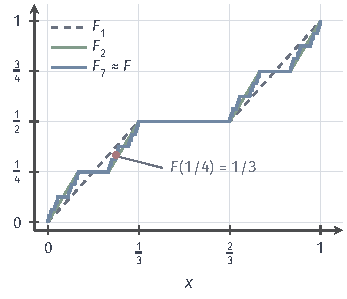
\includegraphics[width=58.815mm]{figures/02-abstract-mathematics/01-metric-and-measure/tikz/c2-cantor-function/figure.pdf}
  \caption{Cantor函数的逐步构造。虚线为$F_1$，绿色为$F_2$，蓝色为$F_7$，后者与极限$F$的一致误差不超过$2^{-7}/3$。每一步只在保留区间上增长，在删去的开区间上保持水平；红点为$F(1/4)=1/3$。}
  \label{fig:measure-cantor-function}
\end{figure}

极限函数$F$称为\term{Cantor函数}（Cantor function），图~\ref{fig:measure-cantor-function}画出了它的近似。它继承了以下性质。第一，$F$单调不减，$F(0)=0$，$F(1)=1$，因为每个$F_n$如此，不等式与等式在逐点极限下保持。第二，$F$连续：任给$\varepsilon>0$，取$n$使$2^{-n}/3<\varepsilon/3$，再由$F_n$连续取$\delta$使$|x-y|<\delta$时$|F_n(x)-F_n(y)|<\varepsilon/3$，则
\[
 |F(x)-F(y)|\le|F(x)-F_n(x)|+|F_n(x)-F_n(y)|+|F_n(y)-F(y)|<\varepsilon .
\]
第三，$F$在每个删去的开区间上为常数：第$k$步删去的开区间位于$C_k$之外，此后每一步都不再修改它上面的值。第四，在$C_n$的每个区间$[a,b]$上，$F(b)-F(a)=2^{-n}$，因为以后的修改都不改变区间端点的值。

\paragraph{Cantor测度}
把$F$延拓到整条实轴：$x<0$时$F(x)=0$，$x>1$时$F(x)=1$。延拓后的$F$连续、单调不减、取有限值，满足第~\ref{sec:measure-construction}节中Lebesgue–Stieltjes构造的条件，于是存在Borel测度$\mu_C$使$\mu_C((a,b])=F(b)-F(a)$。称$\mu_C$为\term{Cantor测度}（Cantor measure）。

它的三条性质都可以用前面的结论直接核对。总质量为$\mu_C(\mathbb R)=\lim_m(F(m)-F(-m))=1$。没有原子：$F$连续，所以$\mu_C(\{x\})=F(x)-F(x-)=0$。集中在$C$上：$\mathbb R\setminus C$是$(-\infty,0)$、$(1,\infty)$与可数个删去的开区间之并；在每个这样的开区间$(a,b)$上$F$为常数，由从下连续性，
\[
 \mu_C((a,b))=\lim_{m\to\infty}\mu_C\bigl((a,b-\tfrac1m]\bigr)=\lim_{m\to\infty}\bigl(F(b-\tfrac1m)-F(a)\bigr)=0,
\]
两条半直线同理；由可数次可加性，$\mu_C(\mathbb R\setminus C)=0$。又$\lambda(C)=0$，所以取$N=C$即得$\mu_C\perp\lambda$。

这样，$\mu_C$是一个非零的奇异连续测度：它的累计函数$F$处处连续，没有任何点质量，却把全部质量放在一个长度为零的集合上。由$F$的第四条性质，$\mu_C$给$C_n$的每个区间$[a,b]$的质量为$F(b)-F(a-)=F(b)-F(a)=2^{-n}$，所以$\mu_C(C_n)=2^n\cdot2^{-n}=1$；同一列集合的长度$(2/3)^n$却趋于零。图~\ref{fig:measure-cantor-mass-length}并排画出这两个数列：长度测度越来越看不见的集合，始终承载着Cantor测度的全部质量。

\begin{figure}[!htbp]
  \centering
  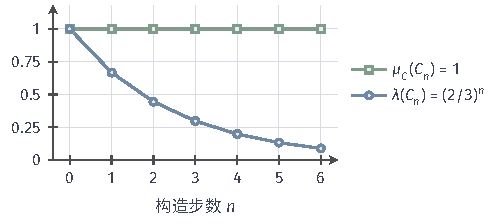
\includegraphics[width=84.691mm]{figures/02-abstract-mathematics/01-metric-and-measure/tikz/c2-cantor-mass-length/figure.pdf}
  \caption{同一列集合$C_n$在两种测度下的质量。蓝色圆点为长度$\lambda(C_n)=(2/3)^n$，$n=0,\dots,6$时从$1$降到约$0.088$；绿色方点为Cantor测度$\mu_C(C_n)=1$，保持不变。由从上连续性，两者的极限分别给出$\lambda(C)=0$与$\mu_C(C)=1$，所以$\mu_C\perp\lambda$。}
  \label{fig:measure-cantor-mass-length}
\end{figure}第~\ref{sec:integral-differentiation}节将再次使用Cantor函数，检验由导数恢复函数增量的公式何时失效。

\paragraph{三类成分的混合}
三种成分可以出现在同一个测度中。令
\[
 \rho=\tfrac12\lambda|_{[0,1]}+\tfrac14\delta_{1/2}+\tfrac14\mu_C .
\]
它是三个有限测度的非负加权和，总质量$\tfrac12+\tfrac14+\tfrac14=1$。累计函数在$[0,1]$上为
\[
 G(x)=\tfrac12x+\tfrac14\mathbf 1_{[1/2,\infty)}(x)+\tfrac14F(x).
\]
由于$1/2$位于删去的区间$(1/3,2/3)$中，$F(1/2)=1/2$，所以$G(1/2-)=\tfrac14+\tfrac18=\tfrac38$，$G(1/2)=\tfrac38+\tfrac14=\tfrac58$，跳跃$\tfrac14$恰是点$1/2$的质量；又如$G(1/4)=\tfrac18+\tfrac1{12}=\tfrac5{24}$。

按定理~\ref{thm:measure-three-part}的步骤分解：唯一的原子是$1/2$，因为$\lambda$与$\mu_C$都没有原子，故$\rho_{\mathrm d}=\tfrac14\delta_{1/2}$；余下的$\tfrac12\lambda|_{[0,1]}+\tfrac14\mu_C$相对于$\lambda$作Lebesgue分解，取$N=C$，前一项在$C$上为零、后一项集中在$C$上，得$\rho_{\mathrm{ac}}=\tfrac12\lambda|_{[0,1]}$，$\rho_{\mathrm{sc}}=\tfrac14\mu_C$。图~\ref{fig:measure-three-part-decomposition}对照了三个分量的累计函数与它们的和。从$G$的图像只能直接读出跳跃；连续增长的部分哪些来自长度、哪些来自Cantor测度，单看“连续”无法区分。第~\ref{chap:densities-change-of-measure}章将用Radon–Nikodym定理说明，绝对连续部分可以由相对于$\lambda$的密度表示，而奇异连续部分不能。

\begin{figure}[!htbp]
  \centering
  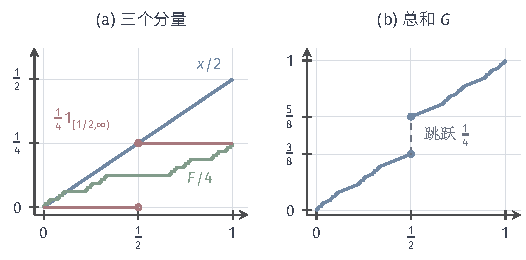
\includegraphics[width=88.999mm]{figures/02-abstract-mathematics/01-metric-and-measure/tikz/c2-three-part-decomposition/figure.pdf}
  \caption{实轴上三类成分的混合$\rho=\tfrac12\lambda|_{[0,1]}+\tfrac14\delta_{1/2}+\tfrac14\mu_C$。(a)三个分量的累计函数：蓝色直线$x/2$来自长度，红色阶跃来自点质量，绿色阶梯状曲线$F/4$来自Cantor测度（以$F_7$近似）。(b)总和$G$在$1/2$处从$3/8$跳到$5/8$，其余部分连续；跳跃对应离散部分，连续增长中既有绝对连续部分，也有奇异连续部分。}
  \label{fig:measure-three-part-decomposition}
\end{figure}

\section{本章小结}
\label{sec:measure-summary}

本章从“集合有多大”出发。第~\ref{sec:measure-size-additivity}节用计数、长度和Jordan测量说明，有限个区间的逼近无法处理有理点集这样的集合，测量规则必须对可数运算封闭。第~\ref{sec:measure-spaces-def}节把问题分成两层：$\sigma$代数规定哪些集合可以测量，测度用可数可加性规定怎样赋值；单调性、次可加性、单调连续性和零测例外都由这两条规定推出。第~\ref{sec:measure-construction}节回答测度从哪里来：外测度把可数覆盖的代价变成集合函数，Carathéodory条件筛出可加的集合，由此得到Lebesgue测度、Lebesgue–Stieltjes测度及一般的延拓定理；$\pi$–$\lambda$定理保证在生成族上一致的测度处处一致。Cantor集说明零测与可数是两回事。第~\ref{sec:measure-measurable-maps}节与第~\ref{sec:measure-pushforward}节转向映射：可测映射让输入端能够回答输出端提出的集合问题，推前测度用原像把输入质量汇集到输出集合上。

同一个Borel结构上可以放置长度、点质量以及它们的混合，因此本章后三节比较同一空间上的不同测度。绝对连续比较零测集是否包含，相互奇异询问质量能否分别集中在互不相交的可测区域；两者都只读取集合质量，相互奇异也不要求距离上的分离。有限测度作差得到有符号测度，Hahn分解找出正负区域，Jordan分解给出唯一的、相互奇异的正负部分，总变差测度$|\eta|$累计不受抵消影响的变化总量。Lebesgue分解则相对于一个参考测度，把$\sigma$有限测度唯一地分成绝对连续部分与奇异部分；在实轴上以Lebesgue测度为参考，奇异部分还能再分成点质量与奇异连续质量，Cantor测度给出后者的具体例子。三种分解分别回答：哪些集合被一同忽略，正负赋值落在哪里，以及相对于参考测度哪些质量能被看见。

进入第~\ref{chap:integration}章时，我们已经有了可测集合、测度、可测函数及其极限运算，简单函数也已定义为可测集合示性函数的有限线性组合；有符号测度的总变差也已就绪。第~\ref{chap:integration}章从简单函数的积分出发，构造简单函数逼近，建立一般积分及其收敛定理。第~\ref{chap:densities-change-of-measure}章在积分可用之后，研究一个测度能否表示为参考测度的加权、怎样计算这种权重并用于换测度。需要强调的是，本章完成的测度分解只把绝对连续质量分了出来，并没有证明它一定能由密度表示；那是Radon–Nikodym定理的任务。

